\documentclass[3p]{elsarticle}
text
\usepackage{lineno,hyperref}
\modulolinenumbers[5]

\usepackage{amsmath, amssymb}
\usepackage[bbgreekl]{mathbbol}
\usepackage{subfig}
\usepackage{wrapfig}
\usepackage{enumerate}
\usepackage{bm}
\usepackage{color}
\usepackage{multirow}

\makeatletter 
  \newcommand\figcaption{\def\@captype{figure}\caption} 
  \newcommand\tabcaption{\def\@captype{table}\caption} 
\makeatother

\journal{Computer Aided Geometric Design}

%% `Elsevier LaTeX' style
\bibliographystyle{elsarticle-num}

\begin{document}


\begin{frontmatter}

\title{Improved Smooth Free-Form Deformation with Sharp Feature Awareness}

\author{Zheqi Lu}

\author{Jieqing Feng\corref{mycorrespondingauthor}}
\cortext[mycorrespondingauthor]{Corresponding author}
\ead{jqfeng@cad.zju.edu.cn}

\address{State Key Lab of CAD\&CG, Zhejiang University, China}

\begin{abstract}
In an smooth free-form deformation~\cite{Cui15} of a polygonal object, the linear geometry, e.g., triangles or planar polygons will be subdivided against a knot box, but it will produce pathological triangles which will contribute to many problem about efficiency and robustness. On the other hand, cui utilize the parallel computing power of the GPU via CUDA, which is limited to NVIDIA hardware. Thus, his method can not be used on neithor AMD GPU nor mobile platform. In this paper, we propose an approach which will be used to clip the original model to avoid pathological case. Moreover, we implement the whole framework of smooth FFD with OpenGL compute shader in order to make it more general. Our subdivision method will produce sub-triangles as regular as possible, but cannot guarantee that each sub-triangle lies in a knot box.Accordingly the method will introduce acceptable errors. However, the trade-off is worthwhile in accordance with Error analysis. We also extend the deformation framework to the mobile phone by the aid of the good across-platfor of OpenGL.
\end{abstract}

\begin{keyword}
smooth FFD\sep sharp feature preserving\sep GPU\sep OpenGL compute shader\sep normal field
\end{keyword}

\end{frontmatter}

\section{Introduction}
%\textcolor{red}{Free-form deformation (FFD) is a prevalent shape manipulation and shape animation method in computer graphics and geometric modeling~\cite{Sederberg86}. Classic FFD is conducted on the sampled points of the geometric model. However, the approach tends to produce an aliased deformation result when using a low sampling density.}

Free-form deformation (FFD\cite{Sederberg86}), as well as many kinds of variants, is useful and widely used whether in academia or in industry when refer to computer graphics and geometric modeling. However, Classic FFD is very simple and efficient but also has many limitation, it is conducted on the sampled points of the geometric model and the approach tends to produce an aliased deformation result when using a low sampling density.

As an alternative, smooth FFD ~\cite{Cui13, Cui14, Cui15} which is on the foundation of accurate FFD (Feng et al., 1998, 2002; Feng and Peng, 2000) deforms the planar polygons as a set of triangular Bézier patches based on the functional composition of Bernstein polynomials (DeRose, 1988; DeRose et al., 1993). The deformation result is smooth and sharp feature awareness. However, In the pre-processing phase, the pathological sub-triangles producted by clip process will worsen efficiency and robustness. So we propose another subdivision approach to get more regular sub-triangles with the cost of a little increase of error. On the other hand, the framework's applicability and generality are bad due to the limit of CUDA. In order to address it, We implement our compute-intensive task with OpenGL compute shader.
The main contributions of the paper are summarized as follows:
\begin{itemize}
    \item A new clip method are proposed to get more regular sub-triangles.
    \item Implement the framework by OpenGL compute shader for better applicability and generality.
\end{itemize}

What's more, graphics applications is move to mobile platform due to the development of mobile hardware. So we also port our work on Android platform. It needs little addition effort thanks to the portable OpenGL.

\section{Related Work}\label{sec:related}

%\textcolor{red}{FFD, which was first proposed by Sederberg and Parry \cite{Sederberg86}, is an intuitive model manipulation and soft
%object animation method. The main concept of FFD is to embed the object into an intermediate space, e.g., a B\'ezier
%volume. Users first edit the shape of the intermediate space; then, the space deformation is transferred to the embedded
%object, whereas the topological connectivity of the object remains unchanged. There are many successive studies
%regarding FFD. Most of these studies focus on improving the interactive means of FFD \cite{Coquillart90, Hui02,
%MacCracken96, McDonnel07, Xu13}. Gain and Bechmann~\cite{Gain08} provided a detailed survey of these methods.}

FFD is an very intuitive method used to deform model or animate soft object. It was first proposed by Sederberg and Parry \cite{Sederberg86} and have inspired many researchers to proposed a series of methods base on the FFD. Gain and Bechmann~\cite{Gain08} provided a detailed survey of these methods. The main idea of FFD is embedding the model into an intermediate space like B\'ezier volume. The intermediate space can be edited by user, then it will transfer the deformation to the embedded model. While the topological connectivity of the model can be reserved during the deformation. However, most of the existing methods focus on the interactive means of FFD but not the quality of the deformation result.

%\textcolor{red}{Traditional FFD and its extensions deform the sampled vertices of the model. Thus, the quality of the deformation result
%depends on the sampling density of the vertex. As a solution to the sampling problem, adaptive upsampling approaches
%\cite{Gain99, Griessmair89, Parry86} are more efficient than the naive uniform upsampling approach on CPU. The adaptive
%upsampling approaches consider the polygon size or surface curvature and upsample the model if necessary. But they
%cannot handle certain special or pathological cases well, and are difficult to be ported on GPU. Accurate FFD, which
%was proposed by Feng et al.~\cite{Feng98, Feng02, Feng00}, is an alternative approach to solving the sampling problem.
%However, it is computationally intensive, and it also consumes considerable bandwidth, i.e., transferring a large amount
%of data from the CPU to the GPU after the intensive computations are performed in the CPU. Thus, the algorithms are not
%interactive or performed in real time in practical applications.}

Traditional FFD deform the sampled vertices of the model as well as its extensions. Therefore, the quality of the deformation result depends on the sampling density of the vertex. To solve the sampling problem, adaptive upsampling approaches \cite{Gain99, Griessmair89, Parry86} are proposed which are more efficient than the naive uniform upsampling approach on CPU. However, they cannot handle certain special or pathological cases well. What's more, it is hard to be ported to GPU. Accurate FFD, proposed by Feng et al.\cite{Feng98, Feng02, Feng00}, is another method to archive high quality of deformed model. But it is not efficient due to intensive computation and also comsumes considerable bandwidth. Thus, the algorithms are not interactive or performed in real time in pratical applications.

%\textcolor{red}{In the recent years, GPUs have been widely adopted for FFD implementations due to their tremendous parallel computing
%power. Chua et al.~\cite{Chua00} proposed an OpenGL-oriented hardware evaluator sub-system to accelerate FFD
%evaluations. However, none of the GPU vendors integrate this type of dedicated sub-system into their GPUs. In contrast,
%GPUs have evolved into general-purpose many-core processors. Schein et al.~\cite{Schein06} implemented a GPU-accelerated
%FFD using the NVIDIA CG language. Jung et al.~\cite{Jung11} achieved the same goal using NVIDIA CUDA and embedded it to
%the X3D system. Hahmann et al.~\cite{Hahmann12} proposed a GPU-based, volume-preserving FFD. They employed the
%multilinear property of volume constraint and derived an explicit solution. The GPU acceleration component implemented
%by CUDA is 6.5-times faster than its CPU counterpart.}

To obtain tremendous parallel computing power, lots of FFD implementations implemented via GPU. Chua et al. \cite{Chua00} proposed an OpenGL-oriented hardware evaluator sub-system specially designed for FFD evaluations. However, GPU parallel computing is developing in the opposite direction. GPU have evolved into general-purpose many-core processors. There're many implementations(\cite{Schein06}, \cite{Jung11}, \cite{Hahmann12}) accelerate FFD via GPGPU. The GPU acceleration component implemented by CUDA is 6.5-times faster thans its CPU counterpart.

%\textcolor{red}{Cui and Feng (2013, 2014) proposed GPU-based accurate FFD of polygonal objects, the results of which are
%represented in terms of trimmed tensor product Bézier patches or triangular Bézier patches. They are sufficiently
%efficient to meet the real-time or interactive demands of large-scale models. However, the deformation is only performed
%on the linear geometry, without considering the normal of the model.}

An accurate FFD of polygonal objects based on GPU is proposed by Cui and Feng(2013, 2014).
Its result is in terms of trimmed tensor product Bézier patches or triangular Bézier patches.
They are efficient enough to meet the real-time or interactive demands of large-scale models.
However, the deformation is only performed on the geometry.
Without considering the normal of the model, the shading effect of the deformed model is unsmooth.

Smooth FFD (Cui and Feng 2015 ) is proposed by Cui and Feng (2015), which adjust the deformed the results of above work according to the normal information of the model so that to obtain a smooth free-form deformation with visually plausible smooth geometry and shading. However, Smooth FFD will generate degenerative triangles and narrow triangle which will do damage accuracy and efficiency in many areas such as CAD, PDE-based computation and so on. And when it comes to generality, Smooth FFD is implemented by CUDA which will limit their whole framework to NVIDIA hardware.

On the other hand, there're more and more graphic applications on the mobile platform. Mobile platform will develop so further that it not only show the 3D things, but also has the demand to edit the 3D model.\cite{mobile1}, \cite{mobile2} already do some work on mobile platform. We want to port a variant FFD method to mobile phone.

Therefore, we propose a method which is based Smooth FFD which can run on multi-platform including mobile platform to address the above problems.

%%%%%%%%%%%%%%%%%%%%%%%%%%%%%%%%%%%%%%%%%%%%%%%%%%%%%%%%%%%%%%%%%%%%

\section{Overview of Accurate FFD in Terms of Triangular B\'ezier Patches}

The GPU-based accurate FFDs~\cite{Cui13, Cui14} of polygonal objects adopt trimmed tensor product B\'ezier patches and
triangular B\'ezier patches as the deformation result, respectively. In this paper, we adopt the framework of accurate
FFD using triangular B\'ezier patches~\cite{Feng98, Feng00, Cui14} since it is more efficient than the one using trimmed
tensor product B\'ezier patches. Some basic notation is introduced below.

$\mathbf R(u,v,w)$ is a B-spline volume of degree $n_u\times n_v\times n_w$ with $m_u\times m_v\times m_w$ control
points:
\begin{equation}
	\footnotesize
	{\mathbf R}(u,v,w) 
	= \sum_{i=0}^{m_u-1}\sum_{j=0}^{m_v-1}\sum_{k=0}^{m_w-1} {\mathbf
	R}_{ijk}N_{i,n_u}(u)N_{j,n_v}(v)N_{k,n_w}(w)
	\label{equ:Ruvw}
\end{equation}

\noindent where $\{\mathbf R_{ijk}\}_{i=0,\hspace{6 pt} j=0,\hspace{8 pt} k=0}^{m_u-1,m_v-1,m_w-1}$ are the control
points, $\{N_{i,n_u}(u)\}_{i=0}^{m_u-1}$, $\{N_{j,n_v}(v)\}_{j=0}^{m_v-1}$ and $\{N_{k,n_w}(w)\}_{k=0}^{m_w-1}$ are
normalized B-spline basis functions, and $\{u_i\}^{n_u+m_u}_{i=0}$, $\{v_i\}^{n_v+m_v}_{j=0}$ and
$\{w_k\}^{n_k+m_k}_{k=0}$ are the knot vectors along the $u$, $v$ and $w$ directions, respectively. Every
three-dimensional region $[u_i, u_{i+1}] \times [v_j, v_{j+1}] \times [w_k, w_{k+1}]$ is called a knot box, where
$n_u\leq i < m_u$, $n_v\leq j < m_v$ and $n_w\leq k < m_w$, respectively.

As described in \cite{Feng98, Feng00, Cui14}, each polygon of the model is first clipped against the knot boxes such
that the generated sub-polygons lie inside of a knot box. Second, the generated sub-polygons are triangulated. The
accurate FFD of such a sub-triangle in a knot box governed by $\mathbf R(u,v,w)$ is a triangular B\'ezier patch
\cite{Feng98, Feng00}, whose degree is $n=n_u+n_v+n_w$. Let the triangular B\'ezier patch be denoted as ${\mathbf
P}(u,v,w)$:

\begin{equation}
	\footnotesize
	{\mathbf P}(u,v,w)
	= \sum_{\substack{i+j+k=n \\ 0\leq i,j,k\leq n}} {\mathbf P}_{ijk}B^n_{ijk}(u,v,w), \hspace{8 pt} u,v,w\ge0,
		\hspace{8 pt}u+v+w=1
	\label{equ:Puvw}
\end{equation}

\noindent where $\{B_{ijk}^n(u,v,w)=\frac{n!}{i!j!k!}u^iv^jw^k \mid i+j+k=n\}$ are the Bernstein basis functions
defined on a 2D simplex, \textit{i.e.}, a triangle. Its control points are $\{\mathbf P_{ijk} \mid i+j+k=n\}$, which
can be efficiently computed via polynomial interpolations \cite{Feng00}.

In Smooth FFD, each triangle and its normal field are deformed as two cubic triangular Bézier patches which are generated via constrained fitting method whose input are the sample points  sampled from B-Spline body. Then, the curved geometry corresponding to the deformed triangles is locally adjusted to tone the smoothness of the geometry appearance according to the deformed normal field. As a result, a smooth free-form deformation with visually plausible smooth geometry and shading is obtained.

\section{Clip Triangle}
%条件数, 数值精度, 零除
The degenerate triangles and skinny triangles generated by clipping against knot cage will have many problem in numerical precision, cross-product for normal, CFD solution and so on.
According to \cite{Feng98, Feng00}, Accurate FFD as well as Smooth FFD will clip the input model against the knot boxes in order to get accurate result of FFD. However, the final result of Smooth FFD is describe as cubic triangular Bézier patch which is only a approximation rather than the accurate high-order one. It is a success trade-off between precision and efficiency. Therefore, the limitation that input model should be clipped against the knot boxes can be remove for the result already not accurate.

Thus, the weakness introduced by bad quality triangle(see \ref{fig:clip_quality}) can also be conquered if we ask for a method which can clip model to triangles as regular as possible rather than clip against knot boxes. On the other side, for two triangles which have the common edge, the clipping scheme generated by our clipping method should be the same on the common edge to avoid cracks.

\begin{figure}
  \centering
  \subfloat[][the clipped model's triangle quality]{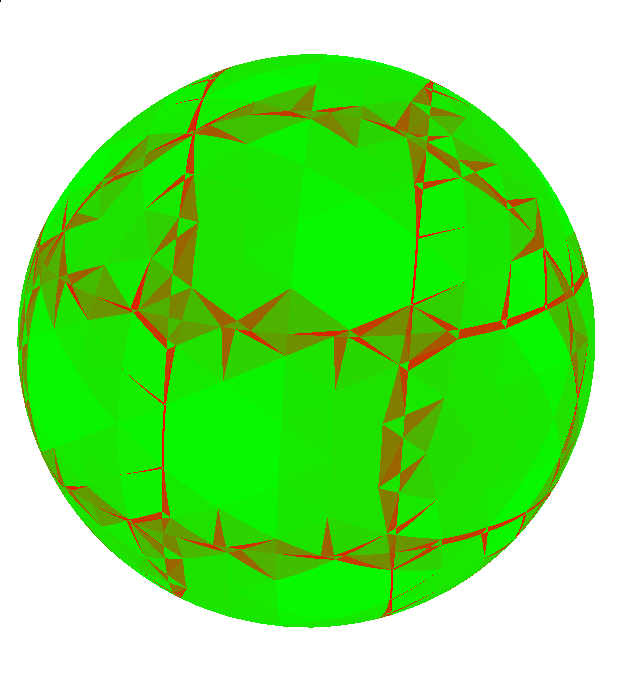
\includegraphics[width=.45\textwidth]{pic/clip_quality1}}\hfill
  \subfloat[][the original model's triangle quality]{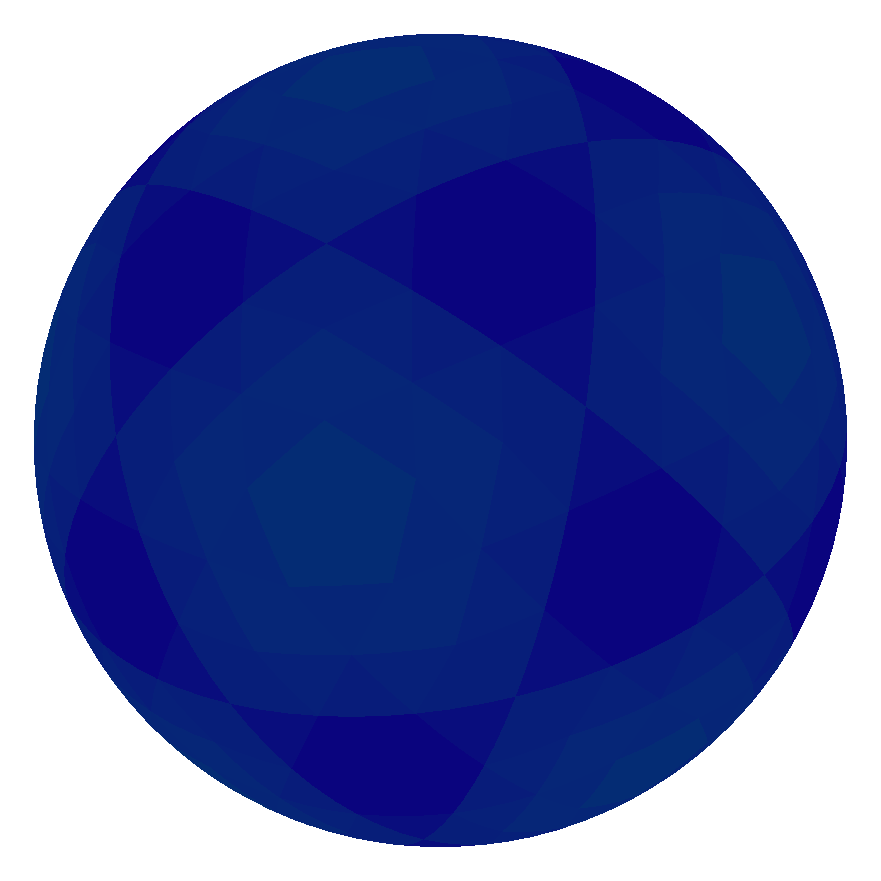
\includegraphics[width=.45\textwidth]{pic/clip_quality2}}\hfill
  \caption{clipping demonstrate}
  \label{fig:clip_quality}
\end{figure}

So our clipping algorithm should archive two goal as follows:
\begin{itemize}
    \item the length of all sub-triangles side should be as equal as possible. Thus, the quality of the sub-triangles is guarantees and the area of sub-triangle will be as similarly to each other as possible.
    \item the adjacent triangles should have the same clip scheme on the common edge to avoid cracks.
\end{itemize}

\subsection{The overview of the clipping algorithm}
In order to satisfy the first goal, we introduce a parameter $l$ as out algorithm's input. All the sub-triangles' edge length should as close to $l$ as possible.

First, we defines some symbols for describing our clip algorithm. $e_i$ is the edges of the Triangle t with $i = 0, 1, 2$. $le_i$ is the length of each edge. Every edge will be clip in to $round(le_i / l)$ segments where l is a constant parameter which can control the size of the sub-triangles and round and length are the round and length function. $p_{ij}$ is the $jth$ point of the $e_i$ generated by previous clip process.
\begin{enumerate}
    \item Find the minimize interior angle of the triangle. We can assume that two sides of the angle is $e_0$, $e_1$.
    \item Compute the clipping points $p_{ij}$ on $e_0$ and $e_1$ which divide corresponding edge into $round(le_i / l)$ segments evenly. $n$ and $m$ is the number of the clipping points of $e_0$ and $e_1$. The indices of clipping points on the two edge are increase from $0$ to $n$ and $m$ along the direction from the vertex whose angle is minimize to the other vertex on the edge. Next, we cut-off the first sub-triangle $e_{00}e_{01}e_{11}$.
    \item The remain part of the triangle is a quadrilateral. We cut off $e_{0i}e_{1i}e_{1(i+1)}e_{0(i+1)}$, segment its edge like step 2 and finally clipping it to sub-triangles. The procedure is iterative. If $n = m$ it repeats for $i$ change from $1$ to $ min(n, m) - 1$ then go to step 5, otherwise $i$ change from $1$ to $min(n, m) - 2$ and go next step.
    \item The remain part is a quadrilateral which is similar to the initial state of step, we can recursively call the process of step 3 until whole input triangle are clipped.
    \item Use CVT method iteratively for 5 times to optimize the position of inner vertexes of the sub-triangles to get more regular sub-triangles.
\end{enumerate}

\begin{figure}
  \centering
  \subfloat[][]{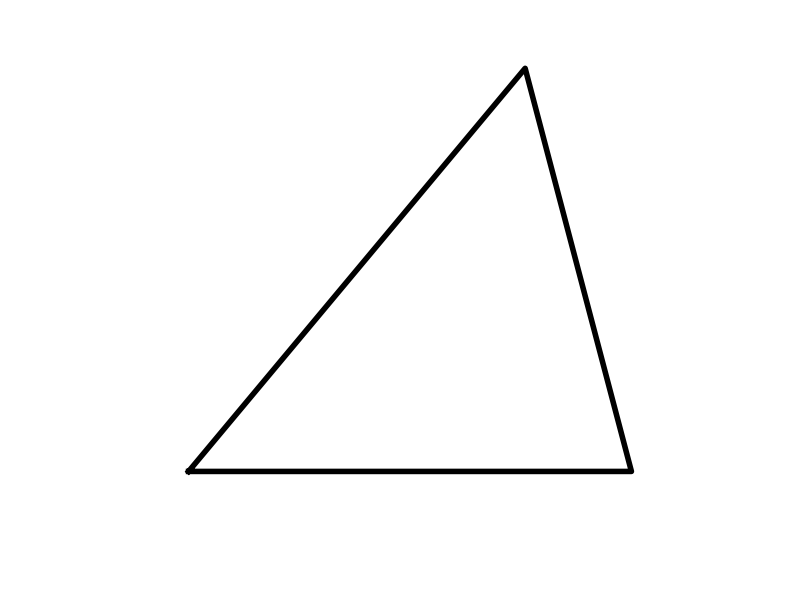
\includegraphics[width=.31\textwidth]{pic/clip_figure0}}\hfill
  \subfloat[][]{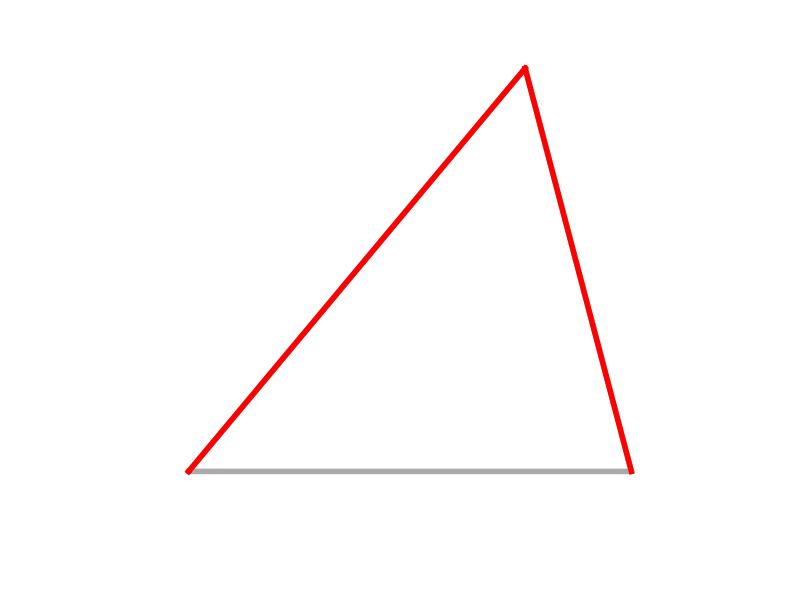
\includegraphics[width=.31\textwidth]{pic/clip_figure1}}\hfill
  \subfloat[][]{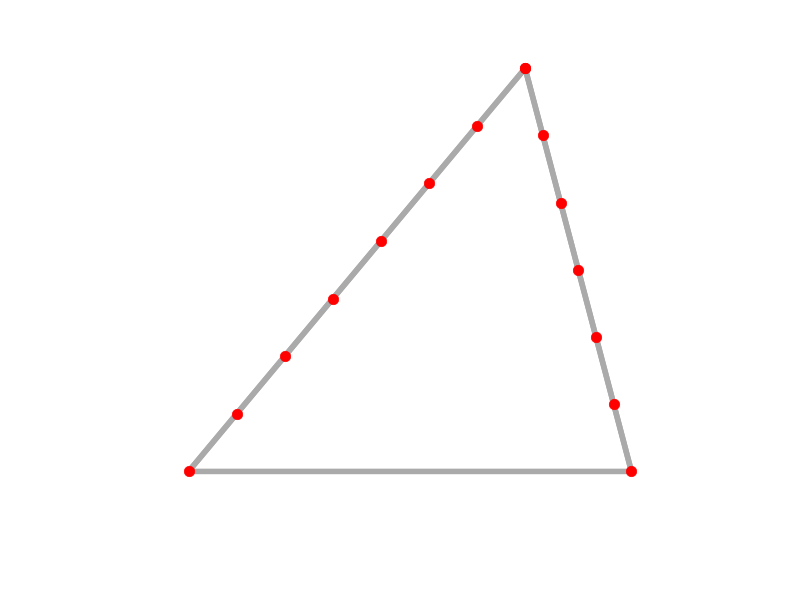
\includegraphics[width=.31\textwidth]{pic/clip_figure2}}\par
  \subfloat[][]{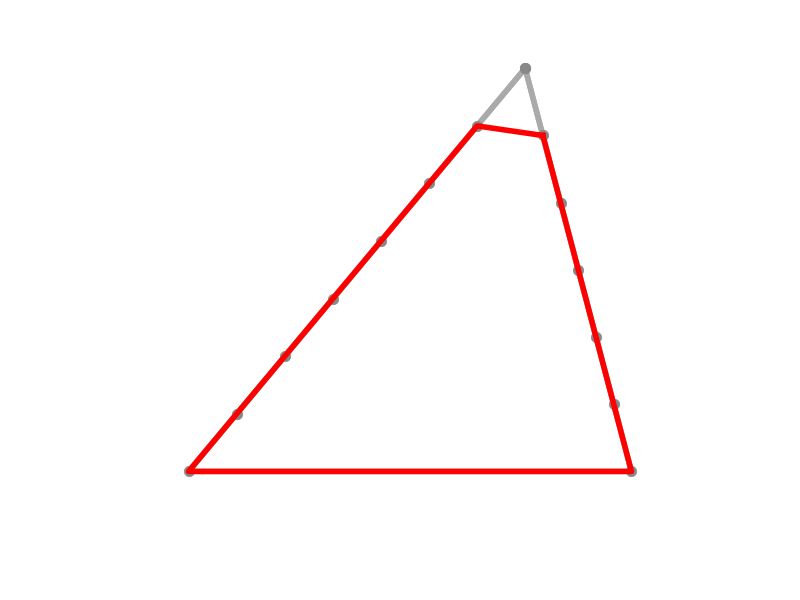
\includegraphics[width=.31\textwidth]{pic/clip_figure3}}\hfill
  \subfloat[][]{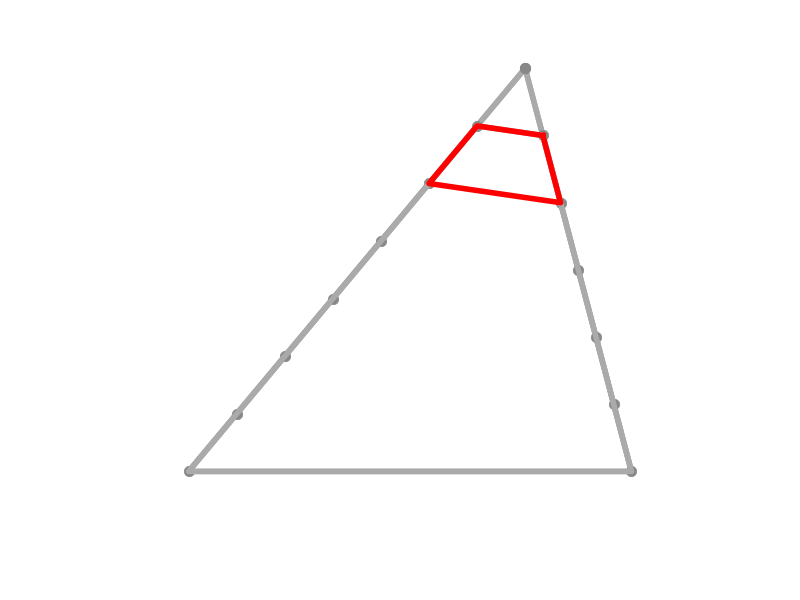
\includegraphics[width=.31\textwidth]{pic/clip_figure4}}\hfill
  \subfloat[][]{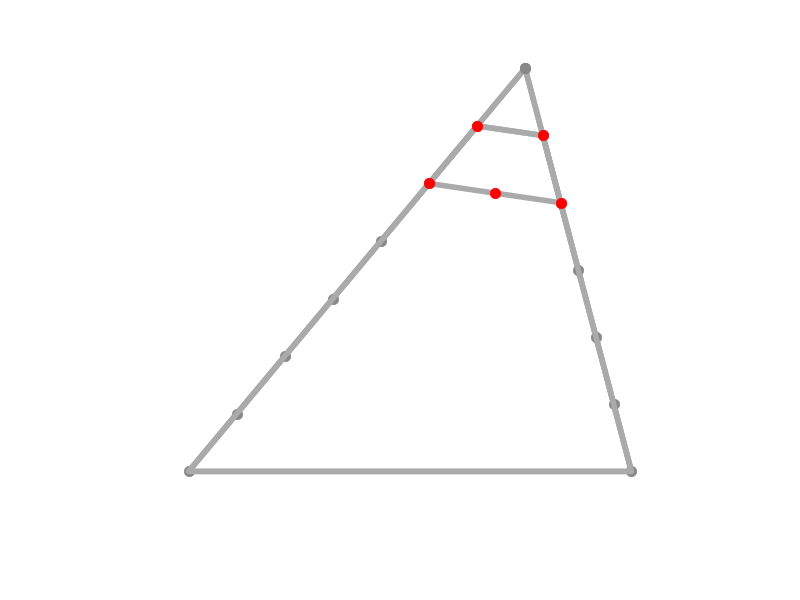
\includegraphics[width=.31\textwidth]{pic/clip_figure5}}\par
  \subfloat[][]{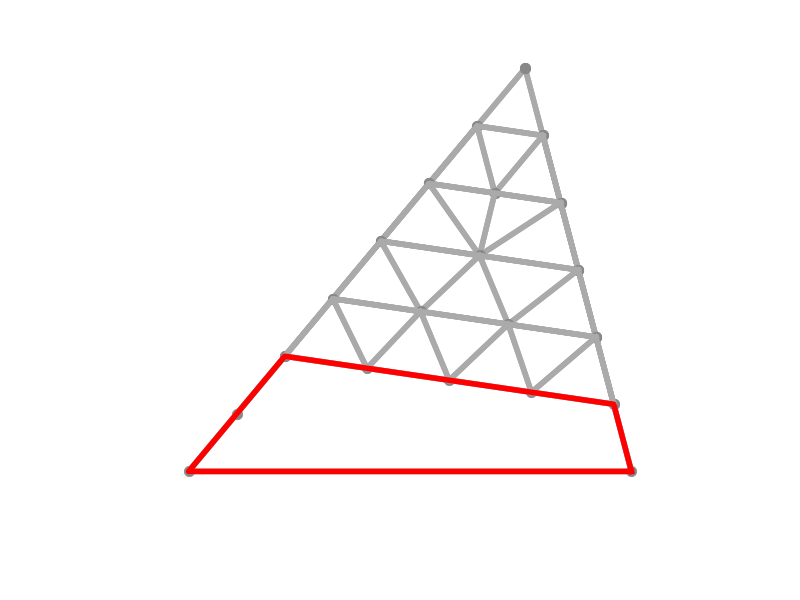
\includegraphics[width=.31\textwidth]{pic/clip_figure16}}\hfill
  \subfloat[][]{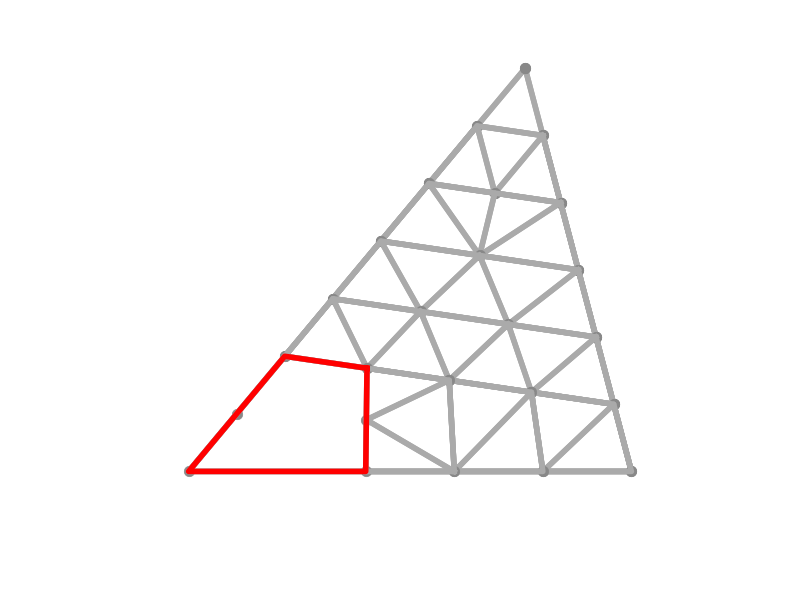
\includegraphics[width=.31\textwidth]{pic/clip_figure26}}\hfill
  \subfloat[][]{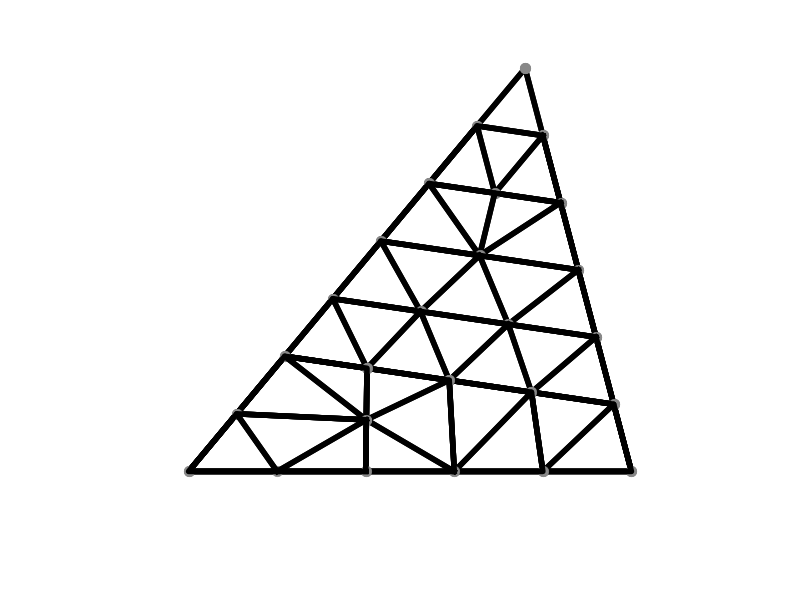
\includegraphics[width=.31\textwidth]{pic/clip_figure33}}\par
  \subfloat[][]{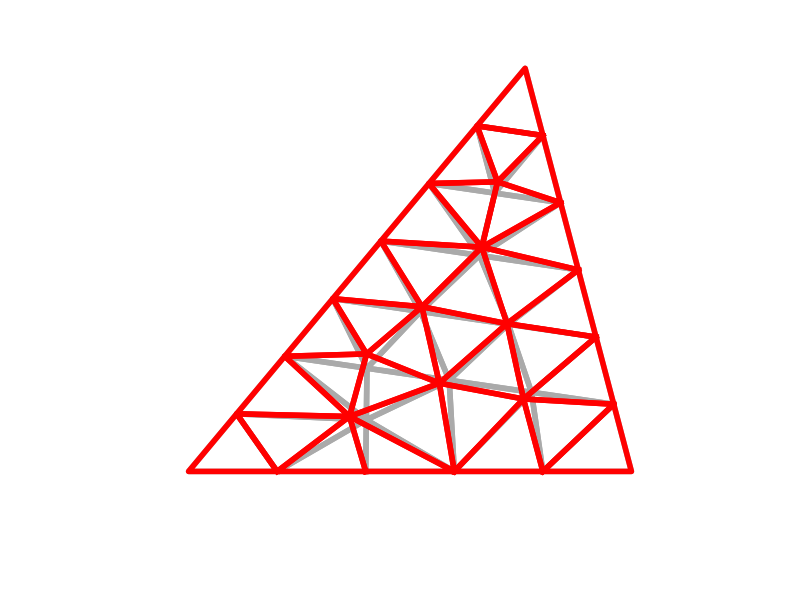
\includegraphics[width=.31\textwidth]{pic/clip_figure34}}
  \caption{clipping demonstrate}
  \label{fig:clip_demonstrate}
\end{figure}

What not mentioned above is some corner case at the end of recursion described in step 3. The last remain part of the triangle maybe can't be handled with step 3. However there's only several corner cases, and we can provide clipping scheme for every of them.

\subsection{the number of iterations}
According to \ref{fig:cvt_iter}, we can see that the improvement of CVT is little after the third time. So we iterative cvt for 5 times.

\begin{figure}
  \centering
  \subfloat[][]{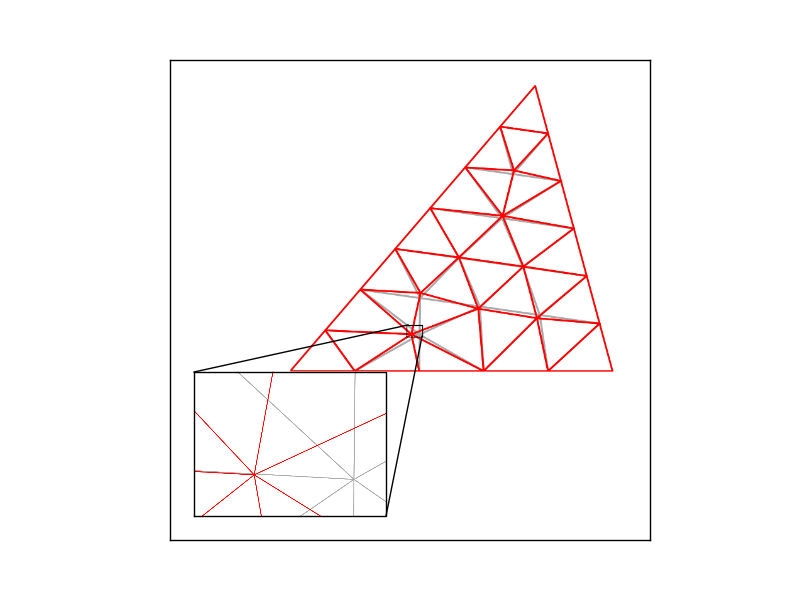
\includegraphics[width=.31\textwidth]{pic/cvt_for_paper0}}\hfill
  \subfloat[][]{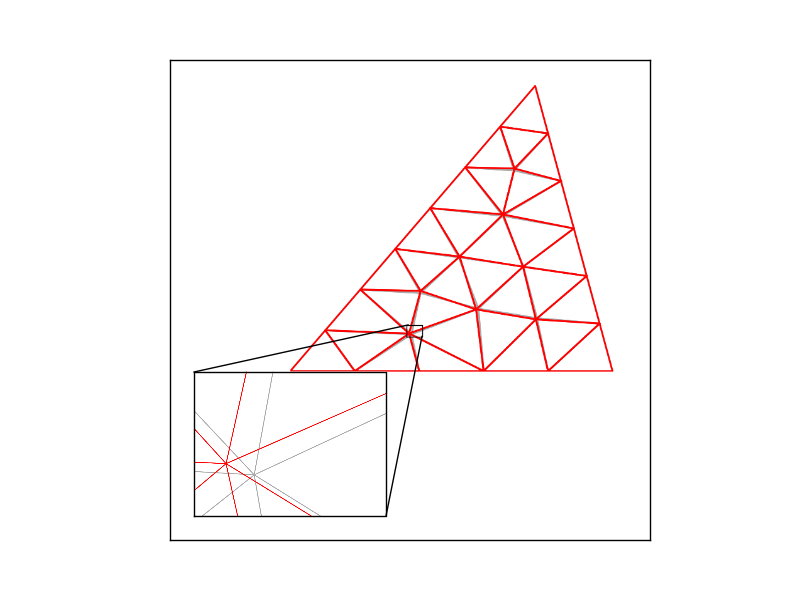
\includegraphics[width=.31\textwidth]{pic/cvt_for_paper1}}\hfill
  \subfloat[][]{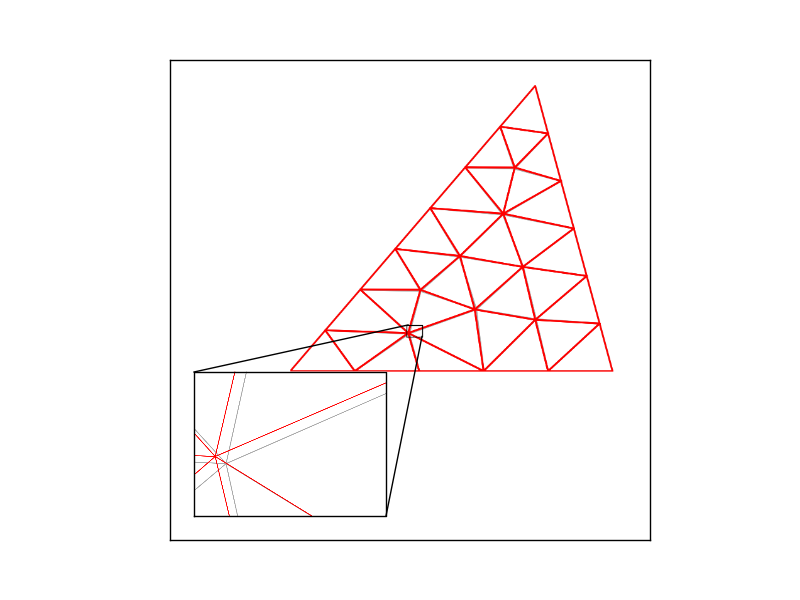
\includegraphics[width=.31\textwidth]{pic/cvt_for_paper2}}\par
  \subfloat[][]{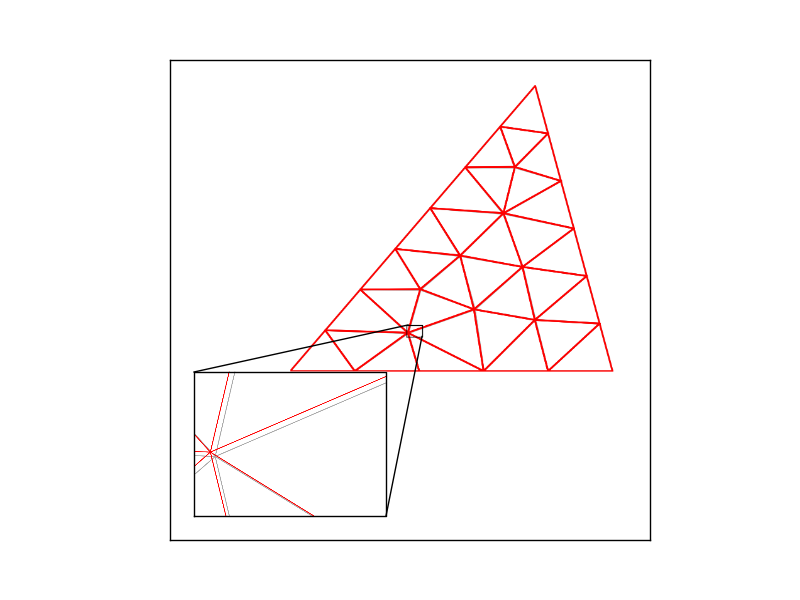
\includegraphics[width=.31\textwidth]{pic/cvt_for_paper3}}\hfill
  \subfloat[][]{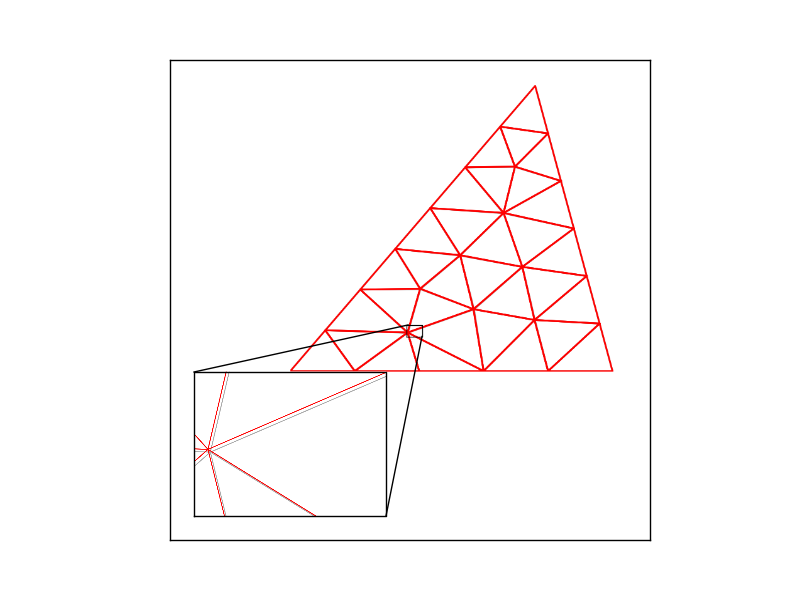
\includegraphics[width=.31\textwidth]{pic/cvt_for_paper4}}\hfill
  \subfloat[][]{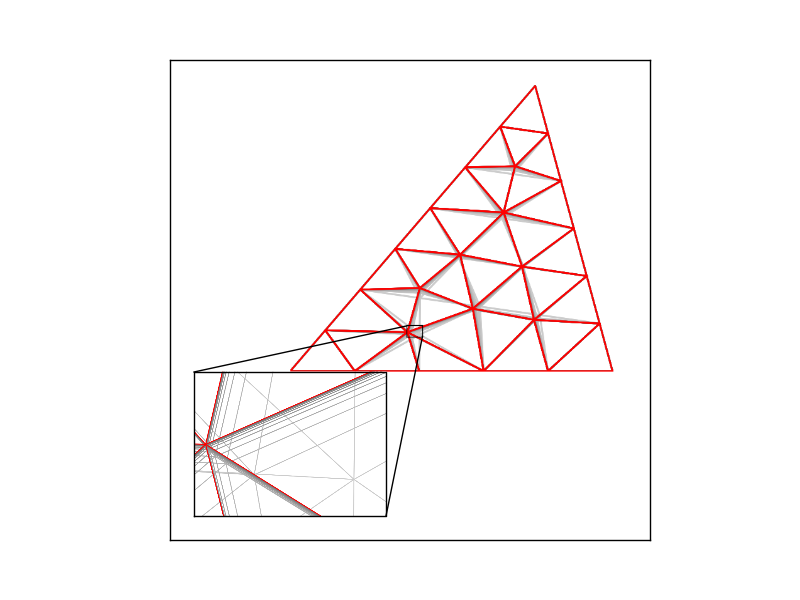
\includegraphics[width=.31\textwidth]{pic/cvt_for_paper5}}\par
  \caption{The red triangles is the result current cvt, The gray is the previous result of cvt}
  \label{fig:cvt_iter}
\end{figure}

\subsection{Some discuss of l}
Our new algorithm will receive a parameter $l$ as the approximate maximum length of the sub-triangles' sides as description above. It is an essential parameter which will effect the number of sub-triangle as well as the error between our final result and Accurate FFD's result. We do a lot of work to find out appropriate $l$ which can minimize the error of the final result for all kinds models from the simple ones formed by a little patches to the fine ones composed by a large number of tiny patches. The result is show in \ref{fig:l_number}, we can find that these is no general $l$ for all kinds of models. However, it can see that the error is had obviously positive correlation with sub-triangle number. What's more, we cannot tell the results of accurate FFD and our method when the l is smaller than the knot cage edge length. So $l$ can be turned from as small as possible to cage size by users according to their demand of accuracy.

\begin{figure}
  \centering
  \subfloat[][]{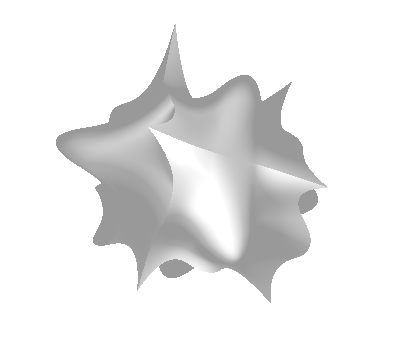
\includegraphics[width=.31\textwidth]{pic/ln_cube_e}}\hfill
  \subfloat[][]{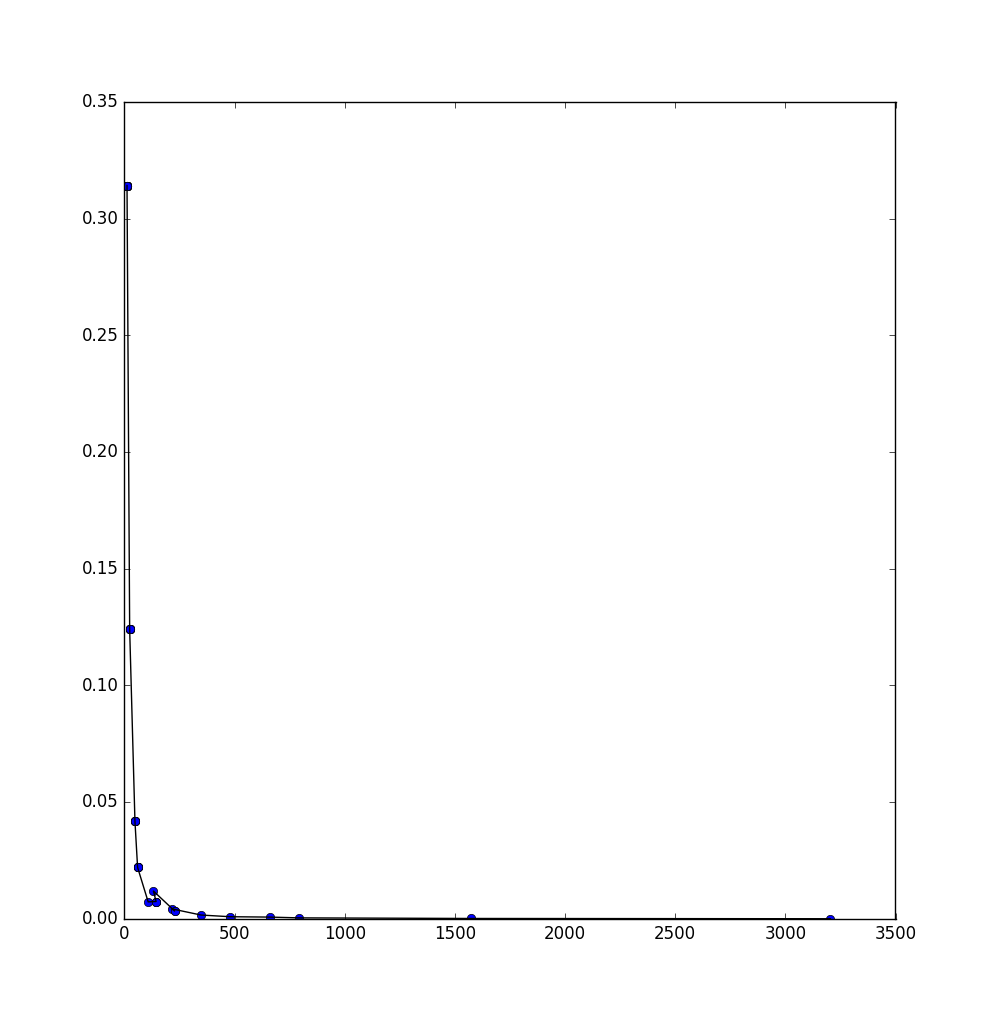
\includegraphics[width=.31\textwidth]{pic/ln_cube}}\hfill
  \subfloat[][]{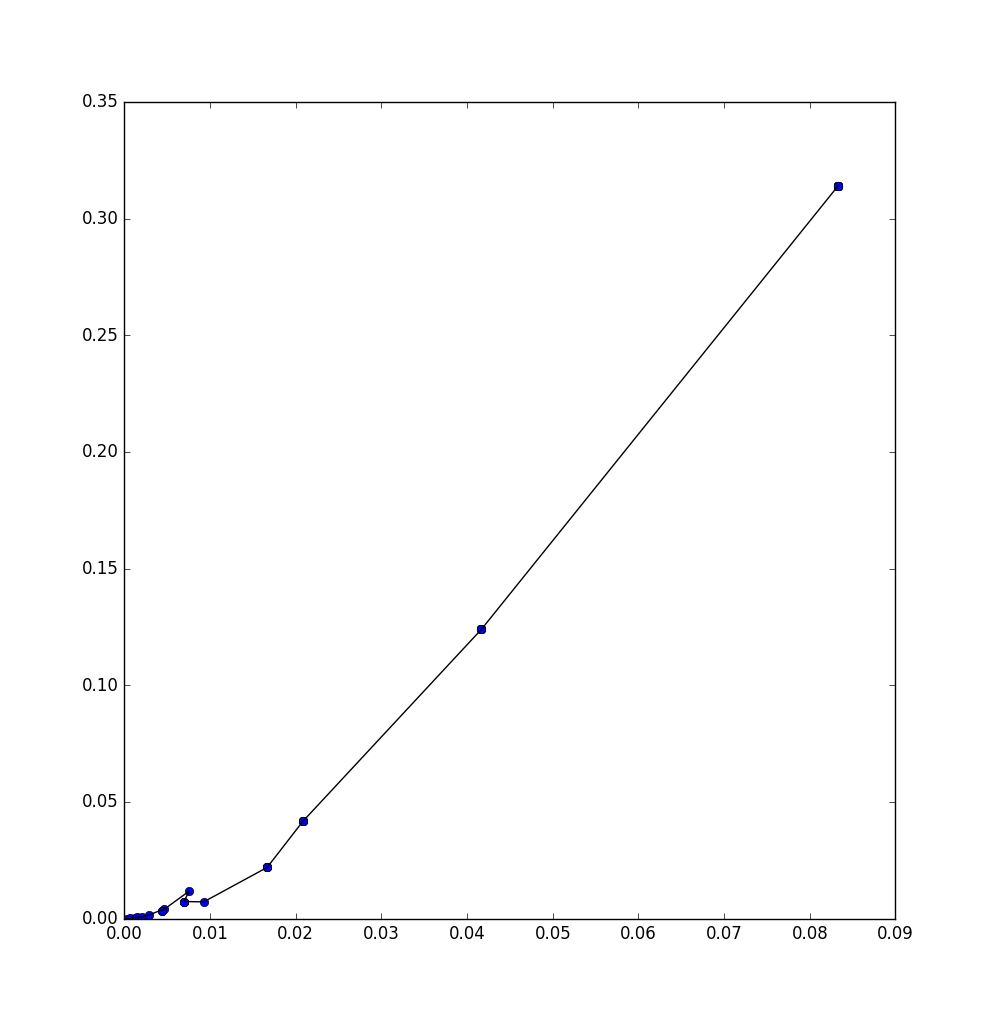
\includegraphics[width=.31\textwidth]{pic/ln_r_cube}}\par
  \subfloat[][]{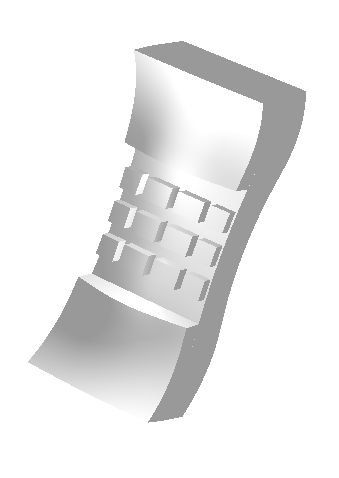
\includegraphics[width=.31\textwidth]{pic/ln_mobile_e}}\hfill
  \subfloat[][]{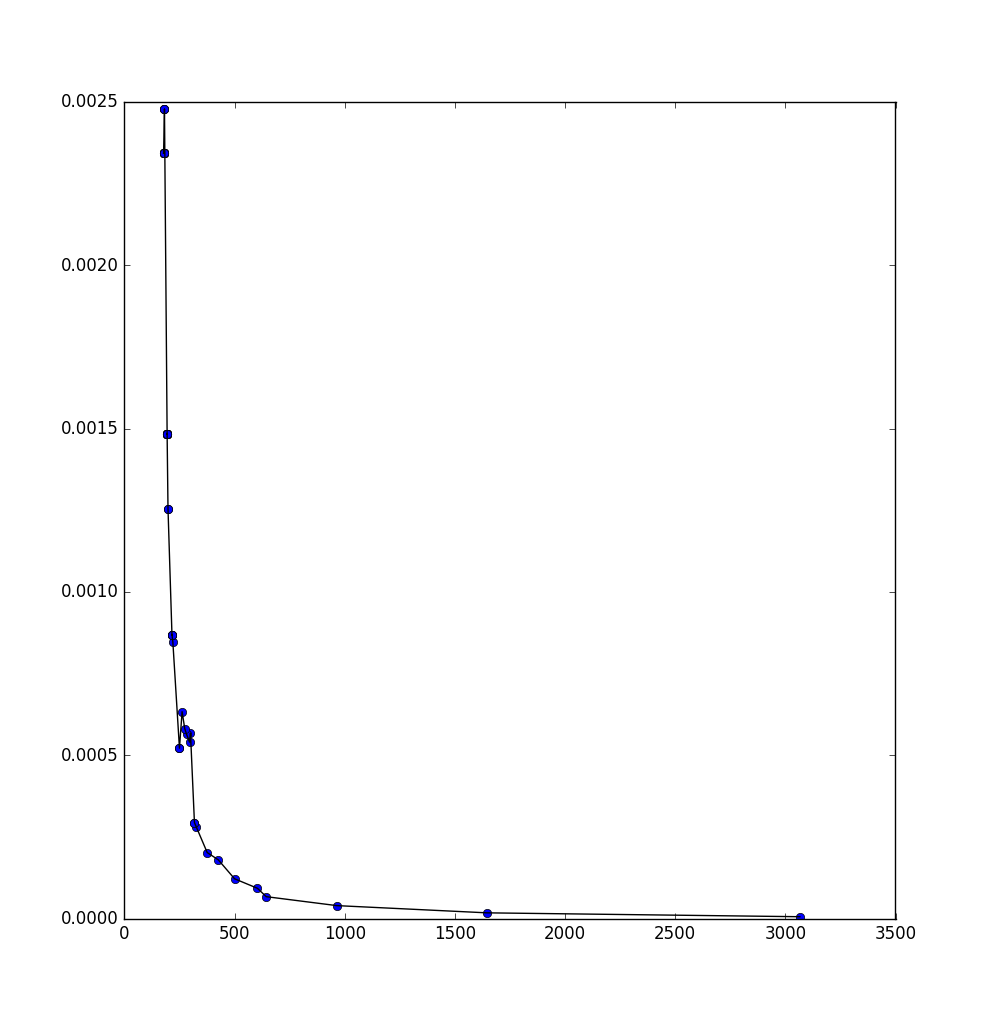
\includegraphics[width=.31\textwidth]{pic/ln_mobile}}\hfill
  \subfloat[][]{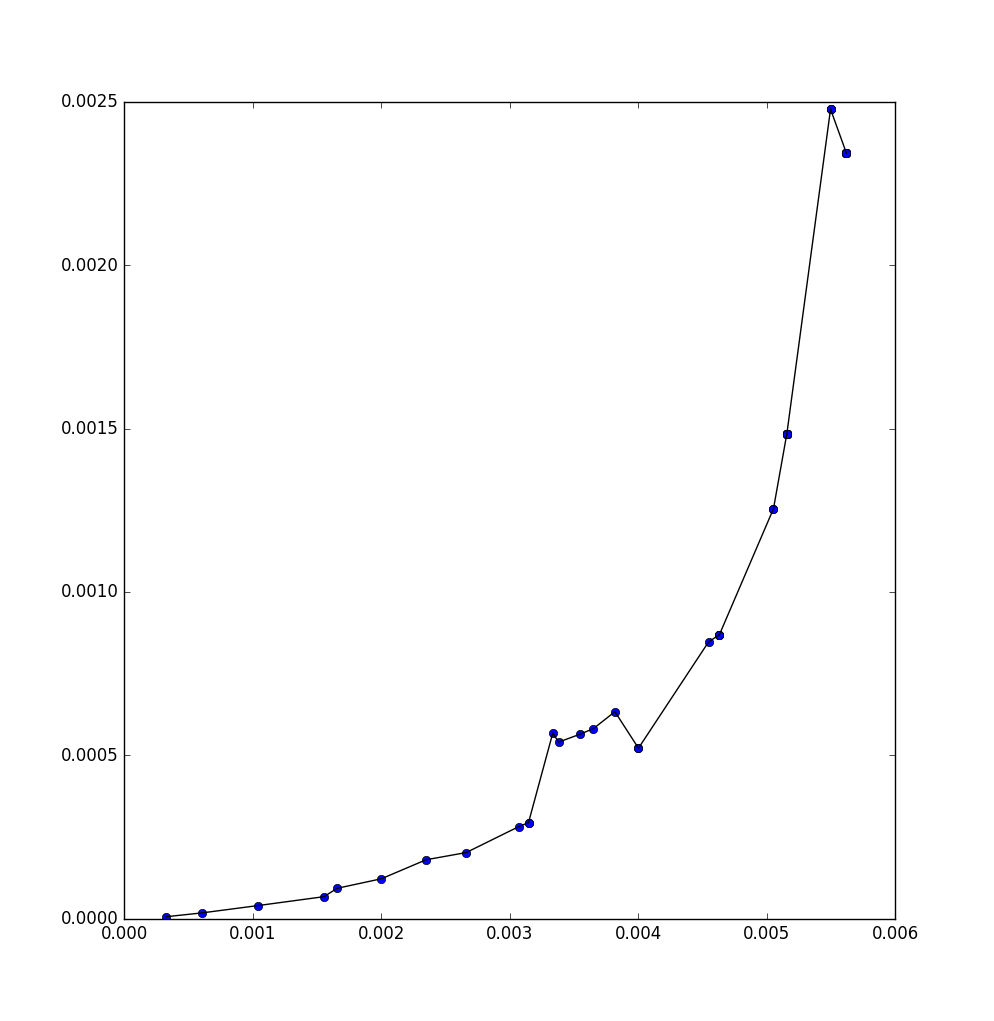
\includegraphics[width=.31\textwidth]{pic/ln_r_mobile}}\par
  \subfloat[][]{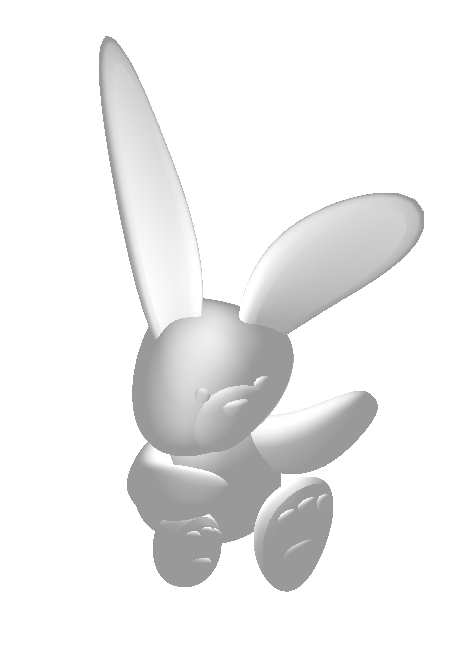
\includegraphics[width=.31\textwidth]{pic/ln_bear_e}}\hfill
  \subfloat[][]{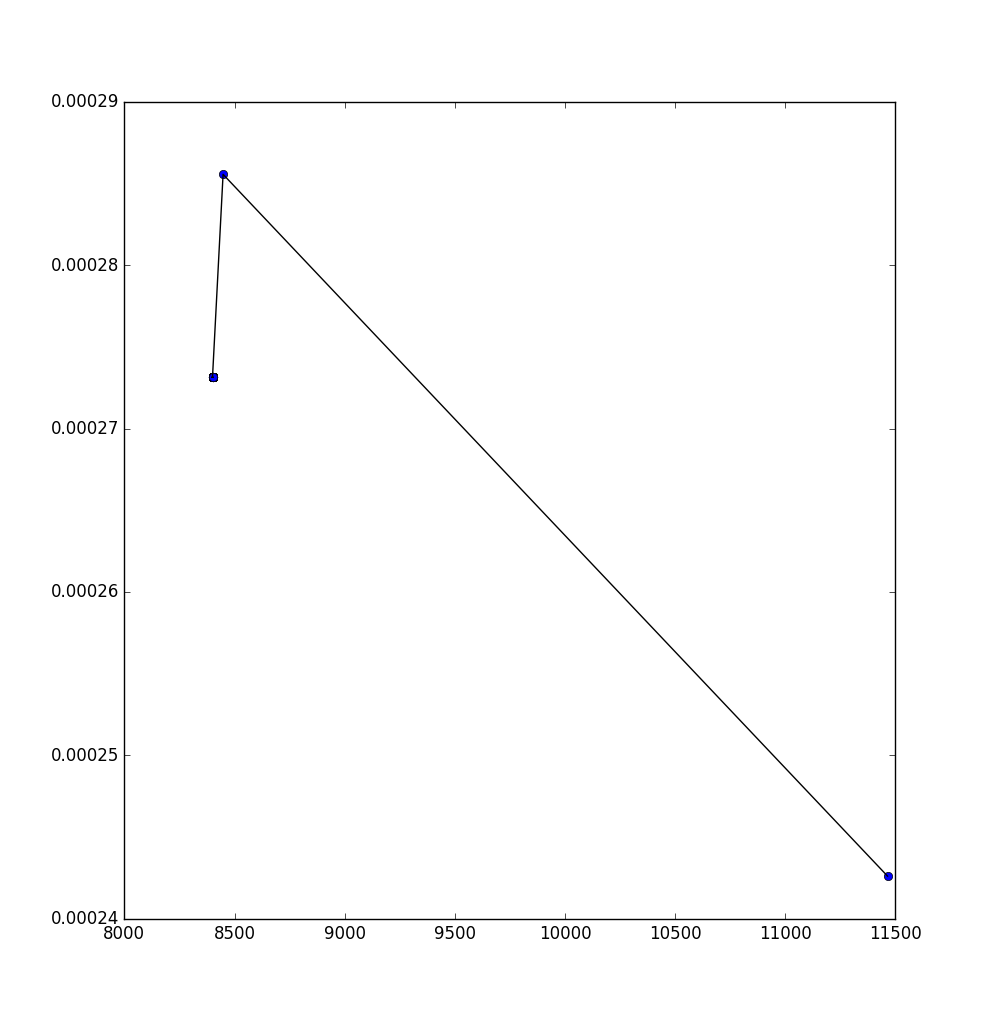
\includegraphics[width=.31\textwidth]{pic/ln_bear}}\hfill
  \subfloat[][]{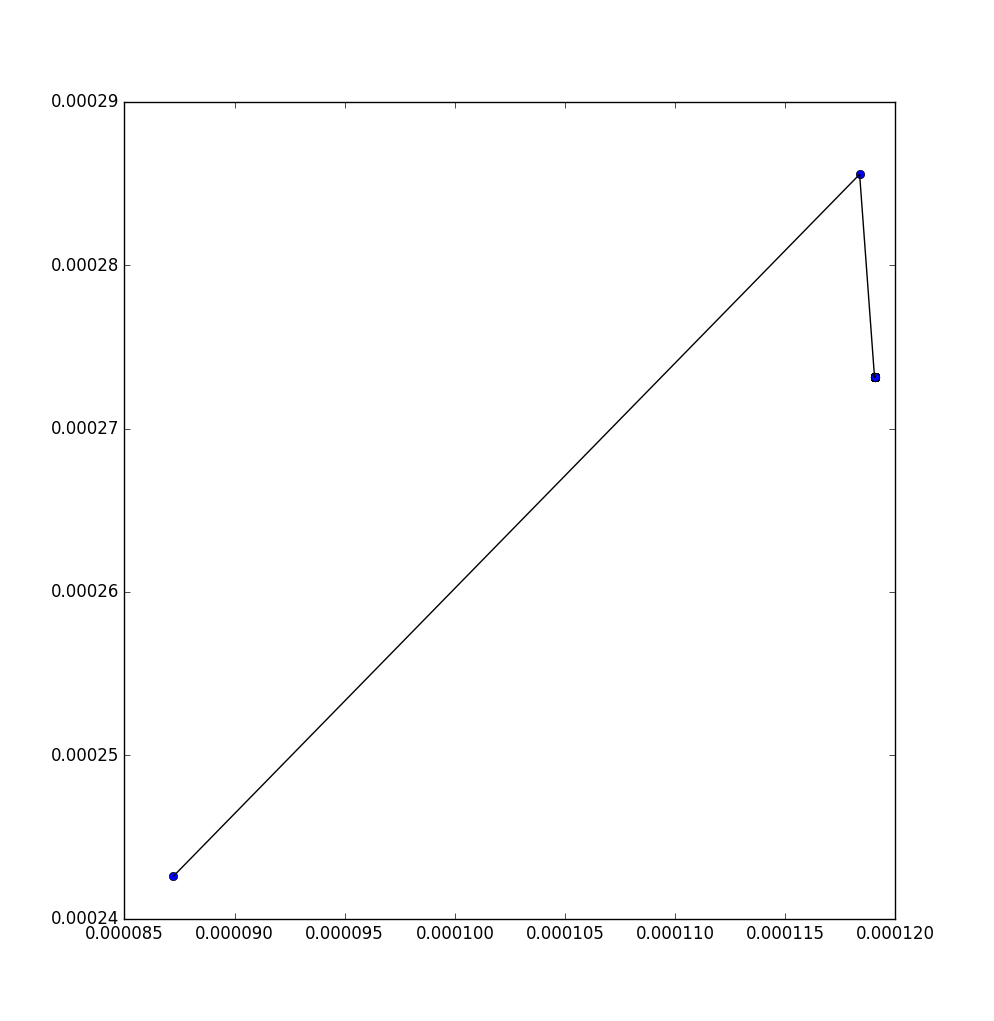
\includegraphics[width=.31\textwidth]{pic/ln_r_bear}}\par
  \caption{Relationship of l and sub-triangles number}
  \label{fig:l_number}
\end{figure}

\subsection{Implement in GPU}
The above algorithm has good result, while it is flexible for different accuracy, but it's to complex to be implemented in OpenGL Compute Shader. Further more, there are a lot of repeated calculation for the model formed by many triangles which have the same size.
Hence, we first compute all possible cases of the clipping of triangles, and restore the result in a table. When we really clip a triangle, we can get a pattern from the table according the size of the triangle and the factor $l$. We trade space for time and the cost of space is reasonable. Of Course, Our GPU clipping triangle algorithm will be faster than the Smooth FFD. The comparison of two algorithm can be see in \ref{tab:compare_pre}.

\section{OpenGL compute shader}
CUDA which is used for implement Smooth FFD is a parallel computing platform and programming model invented by NVIDIA. It enables dramatic increases in computing performance by harnessing the power of the graphics processing unit (GPU). Nevertheless, only on the NVIDIA GPU can CUDA runs. It lead to the compatibility problems in other desktop GPU as well as mobile platform which is rapid developing in recent years.

While Compute Shader is an OpenGL Shader Stage that is used entirely for computing arbitrary information. It is available in every platform as long as it supports OpenGL 4.3.

For this reason, we implement our improved method with OpenGL Compute Shader.

\section{Implementation Results and Comparison}

The proposed method is implemented on a PC with an Intel Core i7 4710MQ CPU@2.50GHz, 8 GB of main memory and an NVIDIA GeForce GT 730M GPU. The operating system is Arch Linux x86\_64. The CPU and GPU components of our method are written using python and OpenGL compute shader, respectively.

We will compare our proposed improved smooth FFD with \cite{Cui15} from the aspects of rendering result, efficiency and approximation errors.

\subsection{Comparison of the rendering results}
\label{sec:comparison_of_rendering}

The deformation results are shown in Figure \ref{fig:ship} and \ref{fig:rabbit}. Each triangular B\'ezier patch is tessellated into 100 triangles. There are 4 sub-figures in each of the 2 examples: (a) is the original model; (b) is the result of smooth FFD \cite{Cui13, Cui14}; (c) is the result of improved smooth FFD; (d) is the textured shading effect of (c).


\begin{figure}[htbp]
\begin{center}
	\begin{minipage}[l]{0.99\textwidth}
		\centering
		\subfloat[]{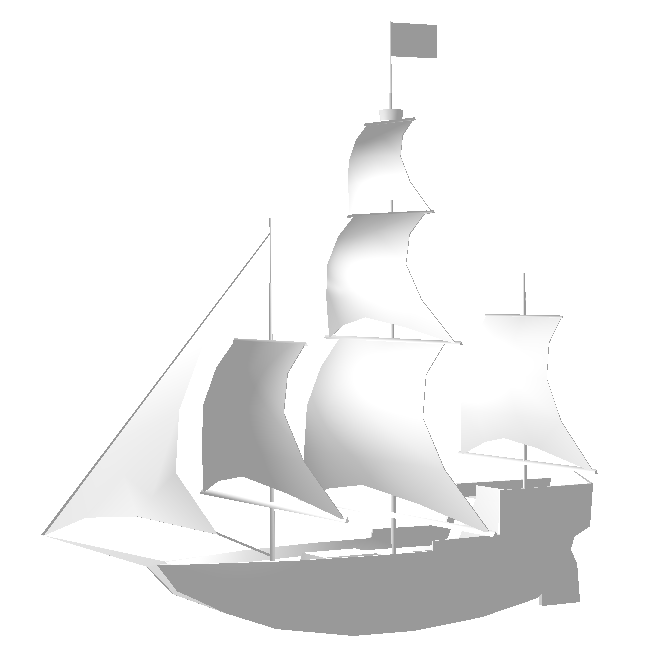
\includegraphics[width=0.24\linewidth]{pic/ship_ori.png}}
		\subfloat[]{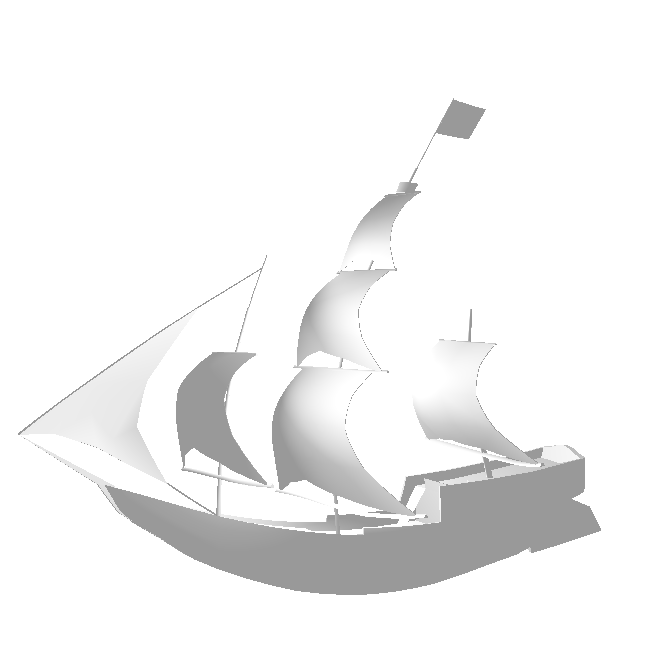
\includegraphics[width=0.24\linewidth]{pic/ship_cym.png}}
		\subfloat[]{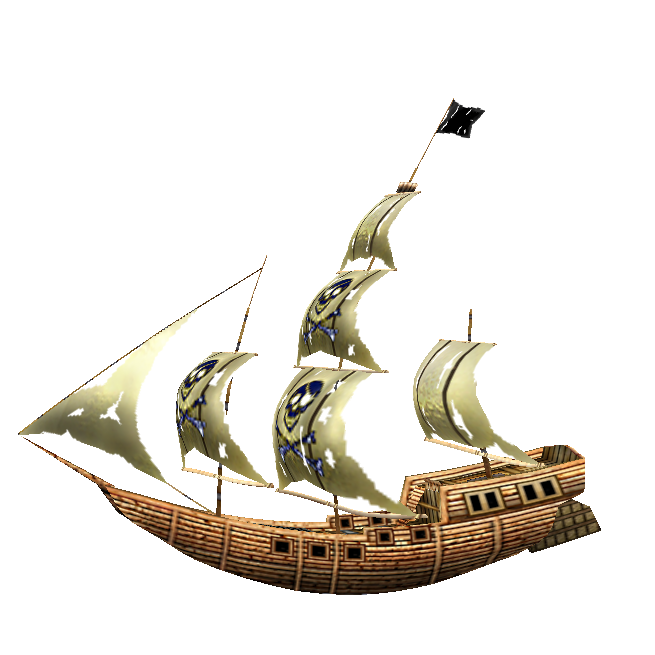
\includegraphics[width=0.24\linewidth]{pic/ship_ac.png}}
		\subfloat[]{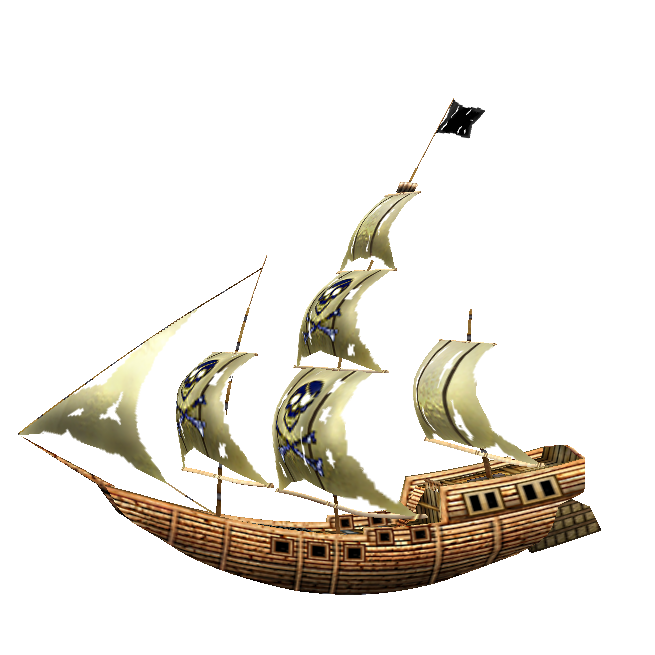
\includegraphics[width=0.24\linewidth]{pic/ship_ac_tex.png}}
		\caption{Deformation of the Ship model by a $3\times3\times3$ B-spline volume with $5\times8\times5$ control points}
		\label{fig:ship}
	\end{minipage}
\end{center}
\end{figure}


\begin{figure}[htbp]
\begin{center}
	\begin{minipage}[c]{0.99\textwidth}
		\centering
		\subfloat[]{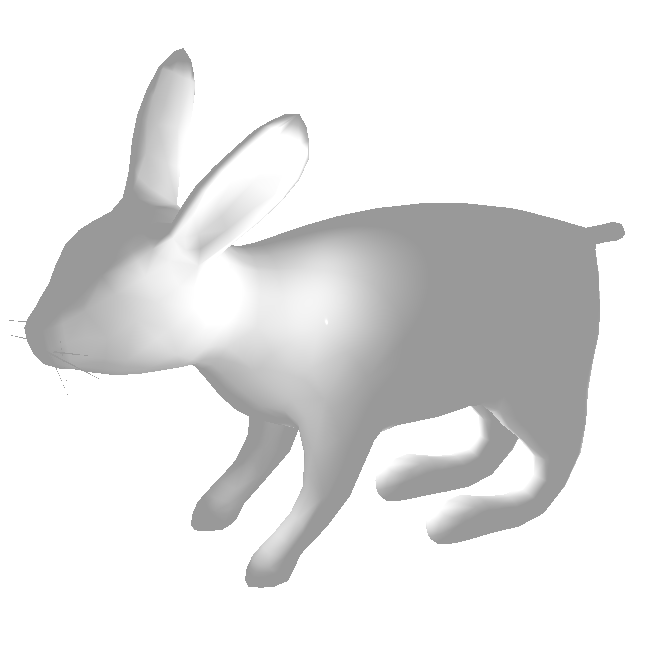
\includegraphics[width=0.242\linewidth]{pic/rabbit_ori.png}}
		\subfloat[]{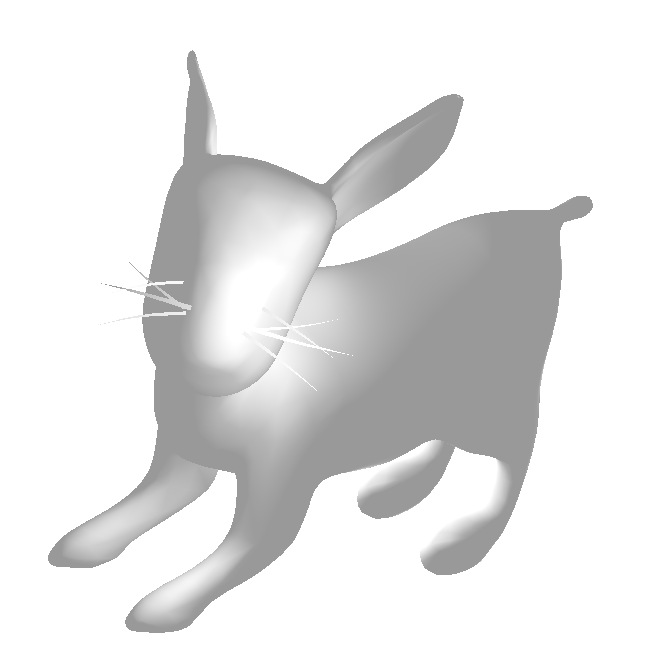
\includegraphics[width=0.242\linewidth]{pic/rabbit_cym.png}}
		\subfloat[]{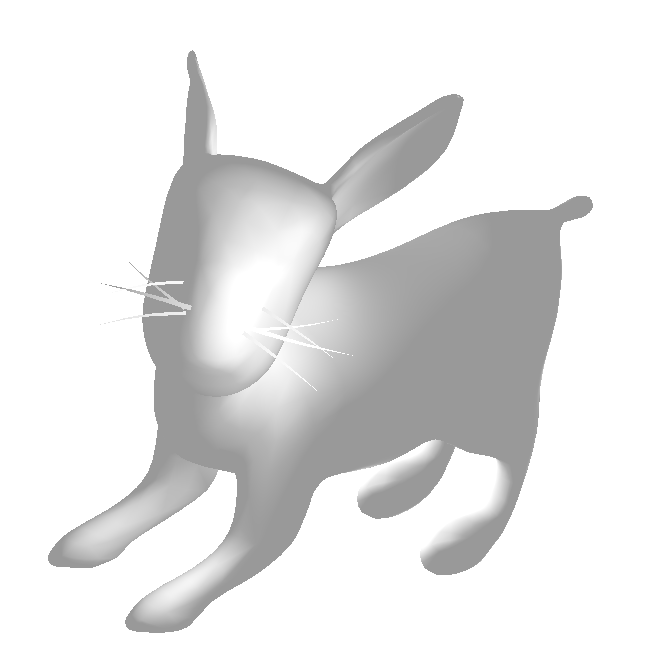
\includegraphics[width=0.242\linewidth]{pic/rabbit_ac.png}}
		\subfloat[]{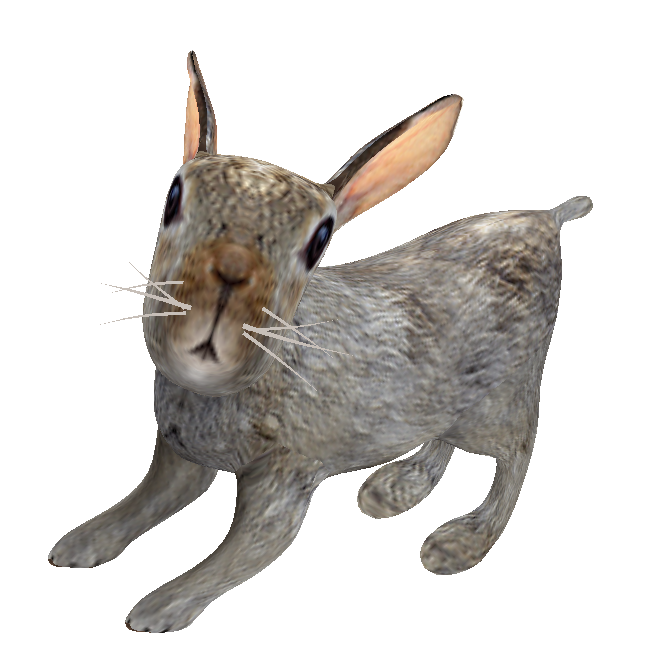
\includegraphics[width=0.242\linewidth]{pic/rabbit_ac_tex.png}}
		\caption{Deformation of the Rabbit model by a $2\times2\times2$ B-spline volume with $5\times8\times5$ control points}
		\label{fig:rabbit}
	\end{minipage}
\end{center}
\end{figure}

These figures illustrate that the results obtained with smooth FFD and improved smooth FFD are almost the same. We can not tell each other with eyes.

\subsection{Comparison of efficiencies}

The efficiencies obtained with improve smooth FFD and \cite{Cui15} are compared in Table \ref{tab:compare_pre} and Table \ref{tab:compare_deform}. The model we use is shown in Figure \ref{fig:snail}. This model has 46,742 faces. As in Section \ref{sec:comparison_of_rendering}, each triangular B\'ezier patch is tessellated into 100 sub-triangles. The degree of the B-spline volume is $2\times2\times2$, with $5\times5\times5$ control points. Table\ref{tab:compare_pre} illustrates that the speed of our method is faster than that of \cite{Cui15} due to clip triangle by GPU which \cite{Cui15} do it by CPU. In the deformation stage, the total time of all stages of Cui's method is 65.464ms. Our method just has an overall run time, 67.419ms, because we implement all of the stages in the same shader while there's not a suitable method to measure time inside a shader. the two method have almost the same efficiencies. The proposed method is sufficiently fast to handle large models in real time.

\begin{figure}
  \centering
  \subfloat[][rendering result of Cui et al.\cite{Cui15}]{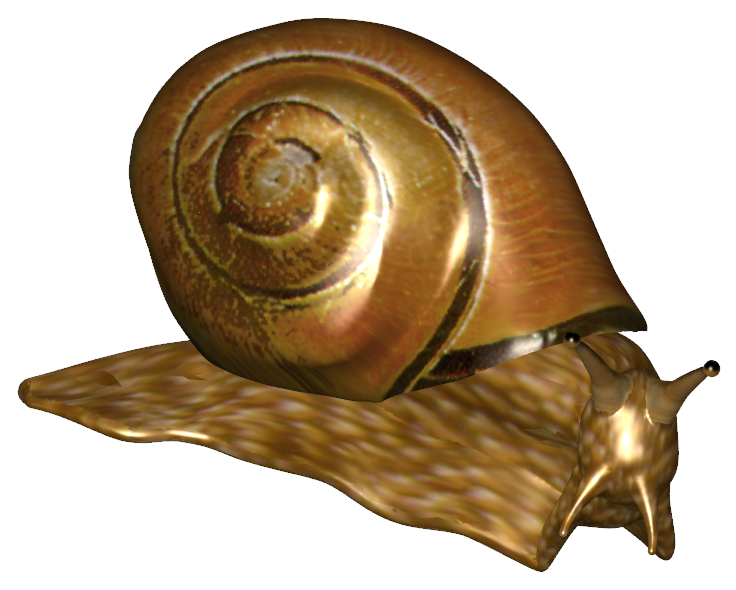
\includegraphics[width=.45\textwidth]{pic/snail1}}\hfill
  \subfloat[][rendering result of our mothod]{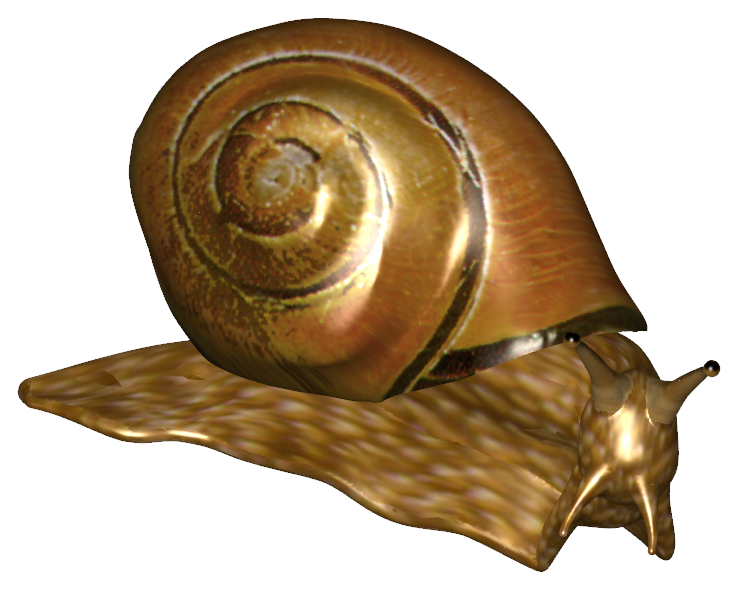
\includegraphics[width=.45\textwidth]{pic/snail2}}\hfill
  \caption{Model used by comparison of efficiencies}
  \label{fig:snail}
\end{figure}

\begin{minipage}[c]{0.99\textwidth} 
  \centering
  \footnotesize
    \tabcaption{Comparison of the efficiencies of our method and \cite{Cui15}(pre-compute stage)}
  \begin{tabular}{llll}
  	\hline
  	Step & Our method & \cite{Cui15}\\
  	\hline
  	Generate PN-triangle         & 4.618   & 104.465     \\
  	Clip triangle                & 21.475  & 5027.418    \\
  	\hline
  	total                        & 26.093  & 5131.883    \\
  	\hline
  \end{tabular}
    \label{tab:compare_pre}
\end{minipage} 

\begin{minipage}[c]{0.99\textwidth} 
  \centering
  \footnotesize
    \tabcaption{Comparison of the efficiencies of our method and \cite{Cui15}(deform stage)}
  \begin{tabular}{llll}
  	\hline
  	Step & Our method & \cite{Cui15}\\
      %%\hline
      %%Copy control points to the GPU    & 0.004   & 0.287     \\
  	\hline
      Calculate the sampling points     & \multirow{6}{*}{67.419} & 30.522     \\
  	Calculate the constraint points   &   & 10.874     \\
  	Calculate the control points      &   & 11.125     \\
  	Calculate the adjusting normals   &   & 4.209     \\
  	Adjust the control points         &   & 4.344     \\
  	Calculate the tessellation points &   & 4.057     \\
  	\hline
  	total                             & 67.419  & 65.464    \\
  	\hline
  \end{tabular}
  \label{tab:compare_deform}
\end{minipage}

\subsection{Approximation error tests}

\begin{figure}
	\centering
    \subfloat[][Original model]{
		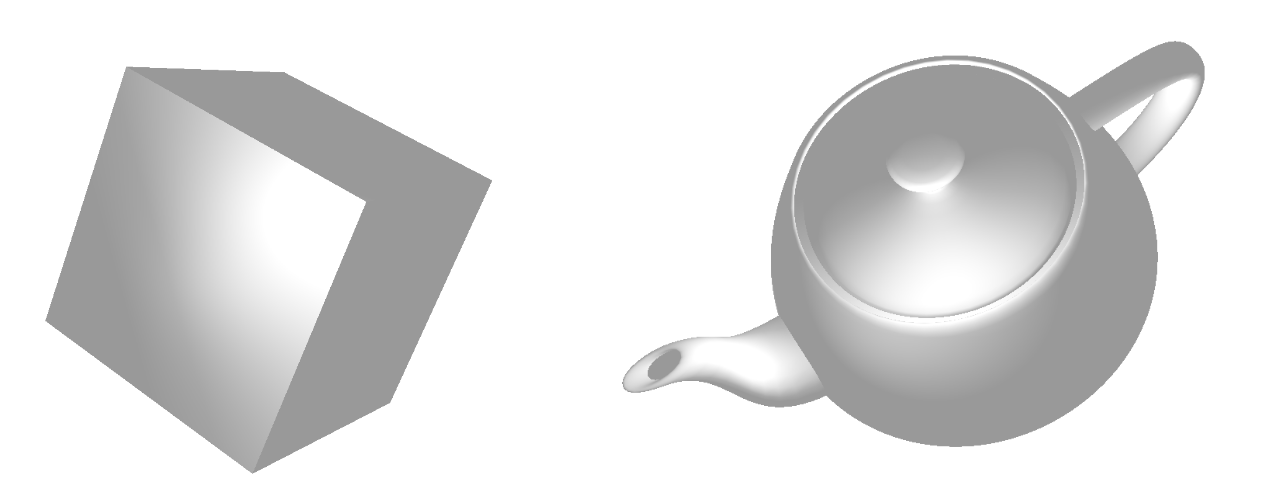
\includegraphics[width=0.99\linewidth]{pic/error0.png}}\par
	\subfloat[][Improved Smooth FFD results of (a)]{
		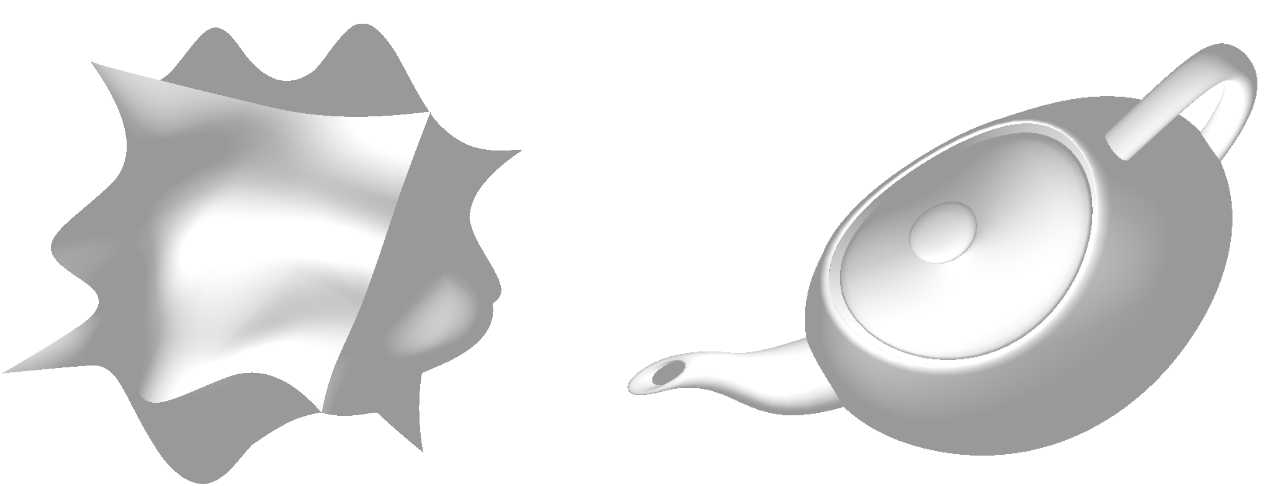
\includegraphics[width=0.99\linewidth]{pic/error2.png}}\par
	\subfloat[][Smooth FFD results of (b)]{
		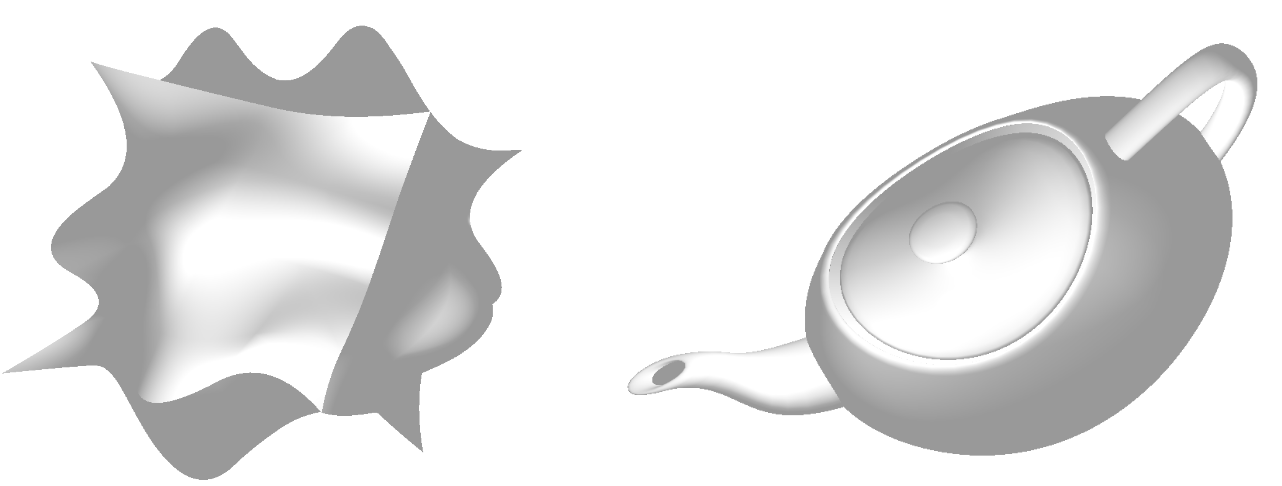
\includegraphics[width=0.99\linewidth]{pic/error3.png}}\par
\end{figure}

\begin{figure}
    \ContinuedFloat
	\subfloat[][Accurate FFD results of (c)]{
		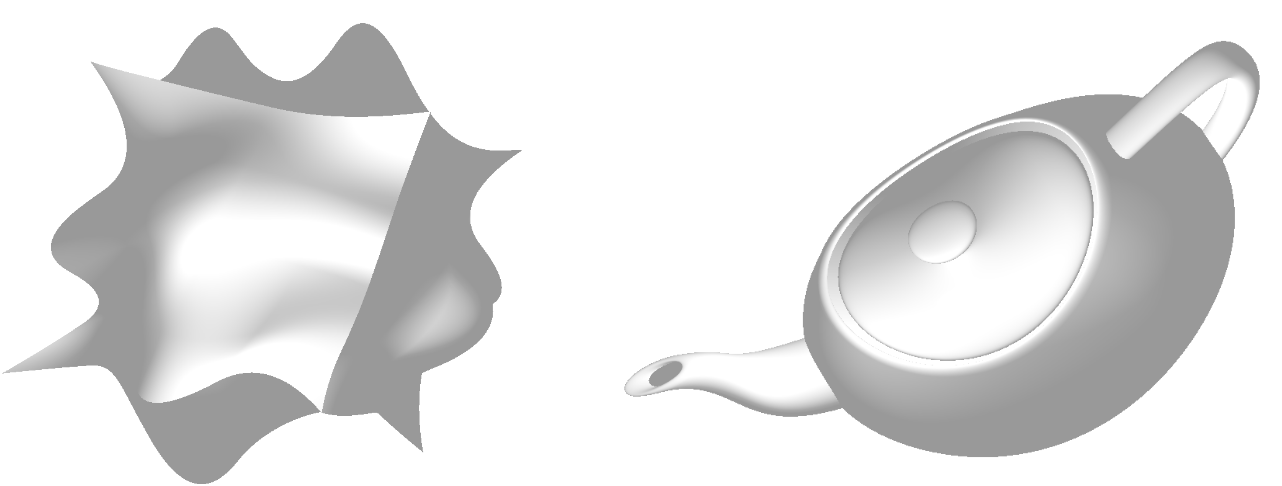
\includegraphics[width=0.99\linewidth]{pic/error1.png}}\par
	\subfloat[][Improved Smooth FFD's Geometry errors]{
		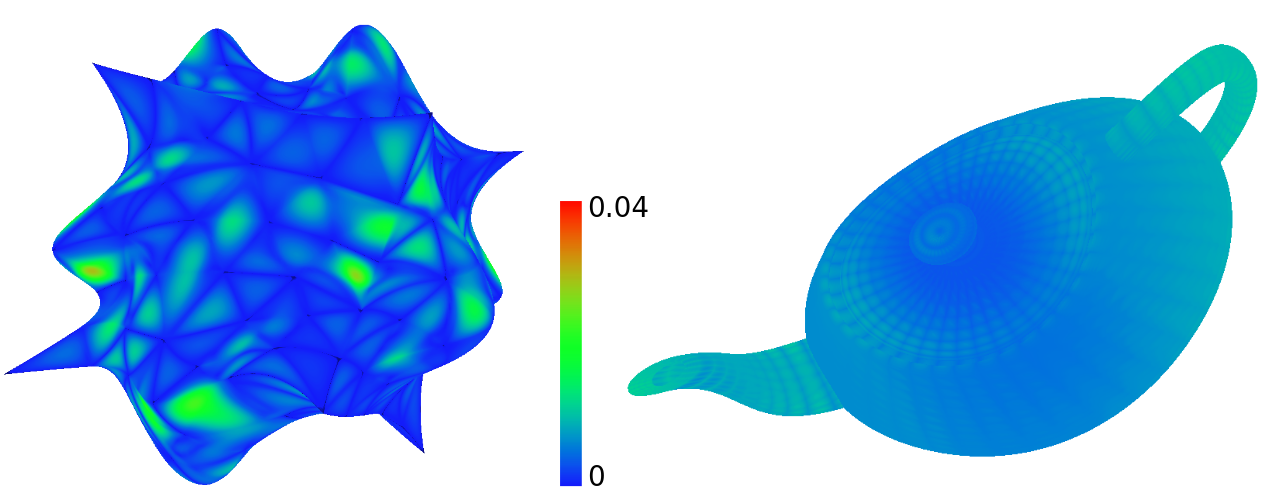
\includegraphics[width=0.99\linewidth]{pic/error4.png}}\par
	\subfloat[][Improved Smooth FFD's Normal errors]{
		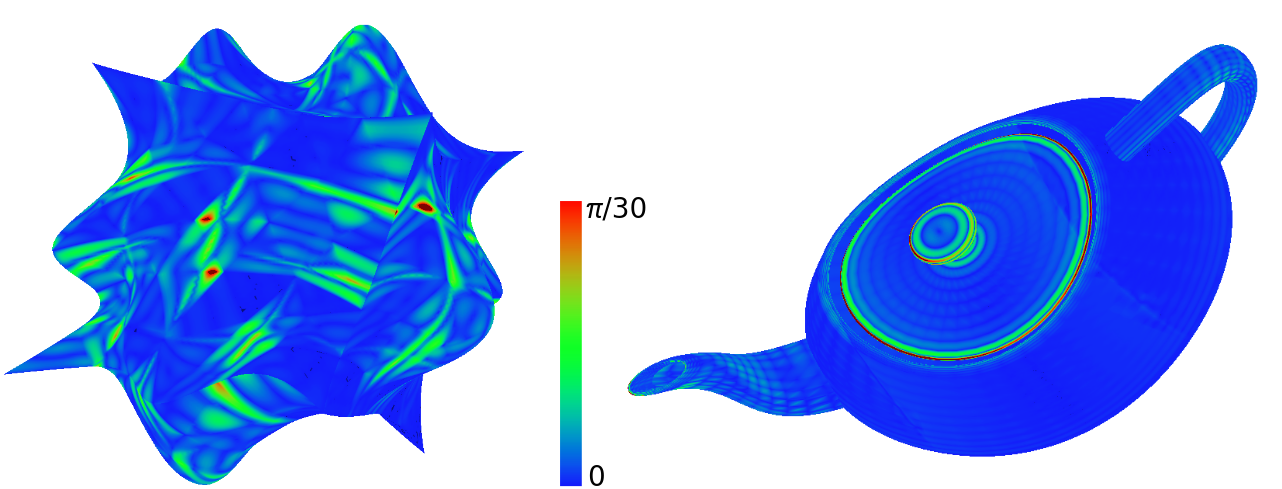
\includegraphics[width=0.99\linewidth]{pic/error5.png}}\par
\end{figure}

\begin{figure}
    \ContinuedFloat
	\subfloat[][Smooth FFD's Geometry errors]{
		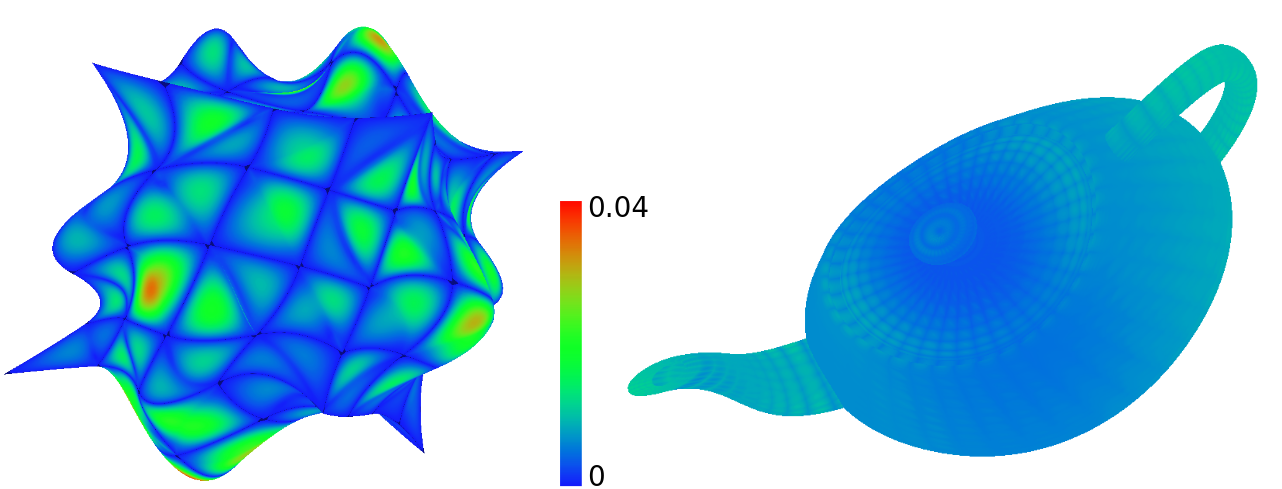
\includegraphics[width=0.99\linewidth]{pic/error6.png}}\par
	\subfloat[][Smooth FFD's Normal errors]{
		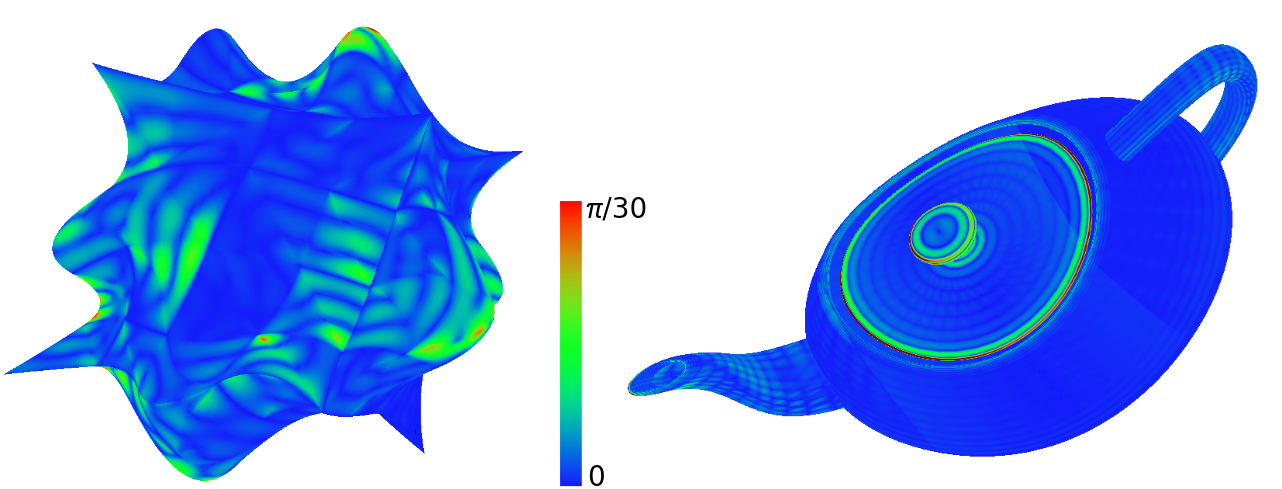
\includegraphics[width=0.99\linewidth]{pic/error7.png}}
	\caption{Error testing}
	\label{fig:error}
\end{figure}

In the improved smooth FFD as well as smooth FFD, both the geometry and normal are obtained approximately via constrained fitting. Thus, there
are approximation errors in the geometry and normal compared with the accurate FFD. Since the smooth parts of a
polygonal object can be regarded as a piecewise linear approximation of a potentially smooth shape, which is unknown in
general, thus it is difficult to evaluate the approximation errors.

Here, we use a Cube model and a Utah teapot model consists of 36 bicubic B\'ezier patches to test the approximation
error, because the geometry and normal of both the input objects are defined accurately. Both of the two models are
normalized into $[-1,1]^3$. The deformations of the Cube model by \cite{Cui13} and \cite{Cui14} are accurate for both
the geometry and normal. The accurate deformation result of Utah teapot is obtained via original FFD of uniformly
sampled points and normals. The input of smooth FFD of the Utah teapot is a mesh generated via de Casteljau
subdivisions. The error test results are shown in Figure\ref{fig:error}, where the first column are the
Cube model deformed by a $2\times2\times2$ B-spline volume, respectively. The second column is the
Utah teapot deformed by a $2\times2\times2$ B-spline volume.

The statistics of geometry error, normal error and volume error are given in Tables~\ref{tab:error_vertex}-\ref{tab:error_volume}, respectively. The geometry error is the Euclidean distances
between the corresponding vertices, and the normal error is the angles between the corresponding normals.


\begin{table}[htbp]
\begin{center}
	\begin{minipage}[c]{0.47\textwidth}
	\footnotesize
	\centering
	\caption{Cube Geometry approximation errors}
	\begin{tabular}{lll}
		\hline
		& Average error & Maximum error \\
		\hline
			Improved Smooth FFD & 0.002952310 & 0.02908119 \\
			Smooth FFD & 0.004904391 & 0.03718415 \\
		\hline
	\end{tabular}
	\label{tab:error_vertex}
	\end{minipage}
	\begin{minipage}[c]{0.52\textwidth}
	\footnotesize
	\centering
	\caption{Cube Normal approximation errors}
	\begin{tabular}{lll}
		\hline
			& Average error & Maximum error \\
		\hline
			Improved Smooth FFD & 0.5785680$^\circ$ & 15.89719$^\circ$ \\
			Smooth FFD & 0.5853341$^\circ$ & 21.24638$^\circ$ \\
		\hline
	\end{tabular}
	\label{tab:error_normal}
	\end{minipage}
\end{center}
\end{table}

\begin{table}[htbp]
\begin{center}
	\begin{minipage}[c]{0.47\textwidth}
	\footnotesize
	\centering
	\caption{Teapot Geometry approximation errors}
	\begin{tabular}{lll}
		\hline
		& Average error & Maximum error \\
		\hline
			Improved Smooth FFD & 0.006597950 & 0.01203453 \\
			Smooth FFD & 0.006650957 & 0.01220984 \\
		\hline
	\end{tabular}
	\label{tab:error_vertex}
	\end{minipage}
	\begin{minipage}[c]{0.52\textwidth}
	\footnotesize
	\centering
	\caption{Teapot Normal approximation errors}
	\begin{tabular}{lll}
		\hline
			& Average error & Maximum error \\
		\hline
			Improved Smooth FFD & 0.6152188$^\circ$ & 22.53011$^\circ$ \\
			Smooth FFD & 0.5491496$^\circ$ & 22.53010$^\circ$ \\
		\hline
	\end{tabular}
	\label{tab:error_normal}
	\end{minipage}
\end{center}
\end{table}

According to Figure~\ref{fig:error} and Table~\ref{tab:error_vertex}, the proposed improved smooth FFD can
generate good approximations of accurate FFD from the geometry, normal. Among them, only maximum
normal error of the Utah teapot model is a little bit large. The maximum errors only occur at the spout end and lip
which are high curvature parts. Here the input mesh of the Utah teapot is obtained via uniform sampling approach, thus
it is not a good polygonal approximation to its original smooth model. It leads to the maximum normal approximation
error as above. That is to say the maximum error comes from the polygonal mesh approximation to the smooth object, which
is out of scope of the paper.

\section{Conclusion and Future Work}

In this paper, we proposed a GPU-based smooth FFD with sharp features awareness that addresses the unsmoothness of the
normal field and the geometry artifact problems in the framework of accurate FFD. The algorithm can produce a
high-quality deformation result. It is a highly parallellizable GPU algorithm and is able to deform a relatively
large-scale model in real time. The algorithm is intuitive and can be implemented easily. It can handle relatively
coarse meshes and generate smooth deformation results.

The approach can still be improved in several aspects. First, the uniform tessellation of the cubic triangular B\'ezier
patches will generate many unnecessary small triangles. An efficient adaptive tessellation algorithm via GPGPU is an
alternative to our method. Second, the approximation error of the smooth FFD for polygonal object is worth to be
analyzed in theory. A feasible error bound is useful to guide the discretization of an smooth object, which is essential
for generating high-quality deformation result.

\section{Acknowledgement}

The authors would like to thank the anonymous reviewers who gave valuable suggestions to improve the quality of the
paper. This work was supported by the National Natural Science Foundation of China under Grant Nos. 61170138 and
61472349.

\section*{References}

\bibliography{MyBib}

\end{document}
